\documentclass[runningheads]{llncs}
%
\usepackage[T1]{fontenc}
\usepackage{newtxtext}
\usepackage[varvw]{newtxmath}
\usepackage{graphicx}
\usepackage{booktabs}
\usepackage{array}
\usepackage{amsmath}
\usepackage{enumitem}
\usepackage{tabularx}
\usepackage{wrapfig}
% ---- experiment-log entries (appendices) ----
% One block per experiment: a bold heading, then one line per field with an
% upright bold label and a hanging indent.
\newcommand{\expprefix}{}
\newenvironment{explog}[2]{%
  \par\addvspace{0.7\baselineskip}%
  \noindent\textbf{Experiment~\expprefix#1: #2}\par\nopagebreak[4]%
  \begin{description}[leftmargin=5.4em,labelwidth=4.9em,labelsep=0.5em,
      align=left,font=\normalfont\small\bfseries,
      topsep=2pt,itemsep=1pt,parsep=0pt,partopsep=0pt]}
  {\end{description}}
% compact stage lists for the architecture descriptions
\newenvironment{stages}
  {\begin{description}[leftmargin=0pt,font=\normalfont\bfseries,
      topsep=3pt,itemsep=2pt,parsep=0pt]}
  {\end{description}}


\begin{document}

\title{CyberAI Cup 2026: Final Architectures, Experimental Logs, and Critical Findings for Packaging Difference Mining, Compliance Auditing, and Flow Classification}

\titlerunning{CyberAI Cup 2026 - AICS Workshop - ICONIP 2026}
\authorrunning{S. Parashar et al.}
\author{
Siddhant Parashar\inst{1}\textsuperscript{*}
\and Piyush Kumar\inst{1}\textsuperscript{*}
\and Mayank Kumar\inst{1}\textsuperscript{*}
\and Manvi Bansal\inst{1}\textsuperscript{*}
\and Mahek Vedant\inst{1}\textsuperscript{*}
\and Ritika Soni\inst{1}\textsuperscript{*}
\and Krish Chauhan\inst{1}\textsuperscript{*}
\and Arsh Abbas Naqvi\inst{1}
\and Arnabi Dutta\inst{1}
\and Mayank Jangid\inst{1}
\and Anil Singh Parihar\inst{1}
}


\institute{
Ethical Hacking and CyberSecurity Lab, Delhi Technological University\\
\email{ehaxdce@gmail.com}
}

\maketitle
\begingroup
\renewcommand{\thefootnote}{*}
\footnotetext{Co-first authors}
\endgroup

%
\begin{abstract}
The CyberAI Cup 2026 comprised three independent tasks: packaging difference
mining, document-grounded compliance auditing, and real-time communication (RTC)
flow classification. This paper describes our solution to each.
For packaging difference mining, we use a Siamese ConvNeXt-Tiny CenterNet that
decodes at stride~2 to resolve marks as small as $8\times8$\,px, trained with
fold-scoped synthetic small-mark pairs and combined with 8-view test-time
augmentation, Weighted Boxes Fusion and a cross-fold ResNet-18 patch verifier.
It achieves \textbf{0.9577} F1, and a recall-ceiling analysis shows that its
out-of-fold candidate set supports up to 0.9801.
For compliance auditing, we map each of 41 checking points to its governing
sections of the Export Control Rules, condensing a 184-section policy into 18
sections, and audit all nine evidence documents of an establishment in a single
full-context Gemini~3.5~Flash call. This reaches \textbf{0.7818} accuracy, and
full-context reasoning outperformed hybrid retrieval (BM25, dense retrieval and
ColBERT reranking) at lower token cost.
For RTC flow classification from only five packets, we blend gradient-boosted
trees with the tabular foundation model TabICL and add a parameter-free decision
rule derived from a separability analysis of audio-only Zoom windows, reaching
\textbf{0.8746} accuracy.
Our solutions achieved an overall score of 0.8714, the mean of the three task
scores, ranking first of 16 teams. We also report the evaluation protocol behind
every estimate, together with the negative results and implementation bugs that
shaped each design.
\end{abstract}

\section{Introduction}
\label{sec:intro}

The CyberAI Cup 2026 posed three unrelated machine-learning problems: finding small
content differences between packaging designs and photographs of the printed product
(Task~1), deciding statutory compliance from several heterogeneous documents with an
LLM (Task~2), and classifying real-time communication flows from five-packet traces
(Task~3). Table~\ref{tab:official} gives our official results.

The approach was the same in every track: build a controlled baseline, locate where
it fails before changing the model, and measure what the competition metric does not
show (recall ceilings in Task~1, per-class and per-element accuracy in Task~2, and an
upper bound set by one inseparable class pair in Task~3). Several conclusions changed
once we examined the complete pipeline, most visibly in Task~1, where two fusion bugs
made test-time augmentation and ensembling look worse than no fusion.

Our contributions are: (i)~three complete systems with official results; (ii)~for
each task, a record of which estimate came from which protocol (out-of-fold, nested,
development set, official); (iii)~negative results and implementation bugs, including
the effect of each on earlier conclusions; and (iv)~the limitations that remain, with
the experiments we did not run.

Sections~\ref{sec:task1}--\ref{sec:task3} describe, for each task, the problem, the
submitted system, the development path that led to it, and the results.
Section~\ref{sec:discussion} draws the lessons common to the three tracks.
Appendices~\ref{app:t1}--\ref{app:t3} contain the full experimental logs, extended
tables and per-task limitations; Exp.~A$n$, B$n$ and C$n$ denote experiment $n$ of
Task~1, 2 and~3.

\begin{table}
\caption{Official test results (team 1665, rank 1 of 16, overall 0.871353, the mean of the three accuracy values) next to our own estimates.}\label{tab:official}
\centering
\small\setlength{\tabcolsep}{4pt}
\begin{tabular}{lcccc>{\raggedright\arraybackslash}p{4.3cm}}
\toprule
Task & Acc. & Prec. & Rec. & F$_\beta$ & Our estimate \\
\midrule
1 & 0.9577 & 0.9656 & 0.9499 & 0.9577 & pooled OOF F1 0.9465; nested 0.9435 \\
2 & 0.7818 & 0.7758 & 0.7818 & 0.7783 & dev accuracy 0.861 (10 cases) \\
3 & 0.8746 & 0.9211 & 0.8746 & 0.883 & CV accuracy 0.8389; macro-F1 0.8318 \\
\bottomrule
\end{tabular}
\end{table}

\section{Task 1: Packaging Material Difference Mining}
\label{sec:task1}

\subsection{Problem and Data}
\label{sec:t1-problem}

Given a clean design template and a photograph of the corresponding printed packaging,
the system must place a box around every genuine content difference between the two.
Because photographs are re-scanned, re-lit and re-toned versions of the template, the
difficulty is not detecting \emph{some} difference but separating genuine content edits
from scan noise, blur and shadow. Predictions are scored by a single \emph{global}
(pooled, not per-image) F1 at IoU~$\geq$~0.5, with a stated target of 0.97. The
organisers report accuracy, precision, recall and F$_\beta$; for our submission accuracy
and F$_\beta$ coincide (0.9577), so we use F1 throughout.

The training set has 200 pairs with 1{,}407 boxes and the test set 100 pairs
(Table~\ref{tab:t1-dataset} in Appendix~\ref{app:t1}). Two properties dominate the
design space: boxes are small (median $22\times22$\,px, with 83 boxes exactly
$8\times8$\,px), and the changes are asymmetric (842 additions, 558 modifications and
no pure deletions).

\subsection{Submitted System}
\label{sec:t1-arch}

\begin{figure}[t]
\centering
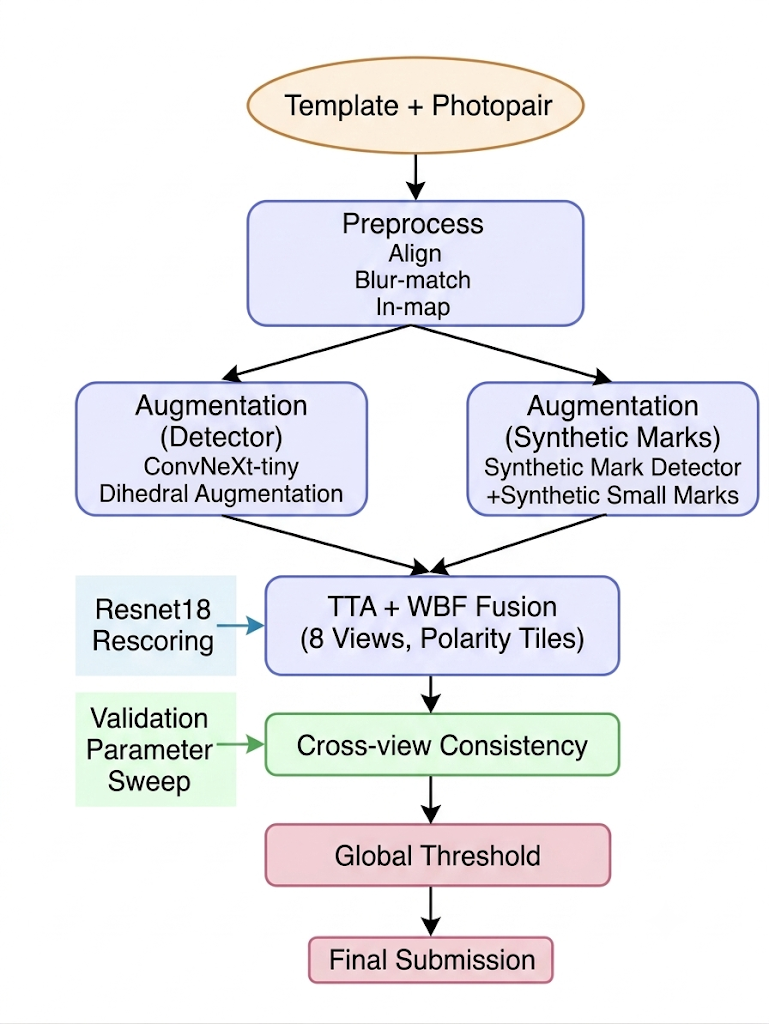
\includegraphics[width=0.38\textwidth]{task1_architecture.png}
\caption{Task~1 pipeline: preprocessing, a ten-detector Siamese CenterNet ensemble,
8-view TTA fused by WBF, five cross-fold ResNet-18 verifiers and the final decode
(threshold 0.43, swept on out-of-fold predictions).}
\label{fig:t1-arch}
\end{figure}

The pipeline (Fig.~\ref{fig:t1-arch}) has five stages.


\noindent\textbf{Stage 0: preprocessing.} A phase-correlation alignment check, with translation
correction if needed; blur matching of the template to the photo by a $\sigma$-grid
search on Laplacian variance; and a shadow- and tone-invariant \emph{ink map},
$\mathrm{GaussianBlur}(\mathrm{gray},\sigma{=}31) - \mathrm{gray}$.

\noindent\textbf{Stage 1: detector.} A Siamese ConvNeXt-Tiny~\cite{liu2022convnext} encoder with
shared weights over 4-channel (BGR~+~ink) streams, fused at every scale by
$\mathrm{conv}(\mathrm{concat}(a,b,|a-b|))$ and decoded through a
U-Net~\cite{ronneberger2015unet} path to \textbf{output stride 2} rather than the usual
4, to resolve the $8\times8$\,px boxes (stride~4 was not ablated). Four
CenterNet-style~\cite{zhou2019centernet} heads predict a centre heatmap, width/height,
a sub-pixel offset and an auxiliary change mask. Two training recipes $\times$ five
folds give ten detectors: \texttt{\_aug} uses the real training pairs with dihedral
augmentation, and \texttt{\_augsyn} adds fold-scoped synthetic small-mark pairs
(Exp.~A5).

\noindent\textbf{Stage 2: TTA fusion.} Each detector runs on 8 dihedral views, fused with Weighted
Boxes Fusion~\cite{solovyev2021wbf}; the detectors' fused outputs are then pooled.

\noindent\textbf{Stage 3: verifier.} A ResNet-18~\cite{he2016resnet} on $96\times96$ crops with an
8-channel stem produces a real-difference probability, blended with the detector
score, and a box-delta refinement. Five verifiers are trained strictly cross-fold.

\noindent\textbf{Stage 4: final decode.} A polarity filter (no pure-deletion class exists in the
data), ink-map snapping with a measured margin, and one global score threshold (0.43),
swept only on out-of-fold predictions.
% TODO: confirm in the code that polarity filter and snapping run after the verifier, as written here

\noindent\textbf{Submission.} The submission contains 668 boxes over the 100 test
images (6.68 per image, against a training average of 7.04), from all ten detectors
with TTA and all five verifiers averaged. The out-of-fold evaluation used a smaller
system (per fold, one detector of each recipe and one verifier), so the official score
is the only estimate that covers the submitted system.

\noindent\textbf{Leakage discipline.} (1)~Synthetic pairs are fold-scoped: each fold
discards the synthetic pairs derived from its own validation pages (836--892 of
6{,}400 per fold). (2)~Unlabelled test templates, which carry no labels, are used as a
synthesis source; no test photographs are used for threshold selection. (3)~The verifier for fold~$k$ trains only on candidates from folds
$\neq k$, produced by detectors that never saw those pages. (4)~The global threshold is
swept on out-of-fold predictions only, never on the reported fold or the test set.
% TODO: confirm that only templates, not test photographs, entered synthesis

\subsection{Development Path}
\label{sec:t1-experiments}

From the first Siamese CenterNet (fold-0 F1 0.9049) to the pooled detector-plus-verifier
system (0.9465), four observations decided the design; Table~\ref{tab:t1-path} in
Appendix~\ref{app:t1} traces every step.


\noindent\textbf{Precision is the hard part.} A classical difference baseline reaches
recall 0.572 but F1 0.0293, because every glyph edge fires in the blurrier photo
(Exp.~A1). Blur matching and the ink map of Stage~0 follow from this.

\noindent\textbf{Model and decode are entangled.} The same \texttt{\_aug} weights
scored 0.9049 at the original decode and 0.9257 with a lower threshold, a larger box
cap and 8-view TTA (Exp.~A6), so earlier ``no gain'' verdicts had compared decoders as
much as models.

\noindent\textbf{The recall ceiling, not F1, chose the ensemble.} The fraction of
ground-truth boxes present anywhere in the candidate list bounds every rescoring
idea. \texttt{\_augsyn} has worse standalone F1 (0.896 against 0.926) but raises the
ceiling from 0.9440 to 0.9590, and on boxes under 12\,px from 0.891 to 0.922
(Exps.~A5, A8). The two-family ensemble adds only 0.001 F1 but lifts the ceiling to
0.963, leaving the verifier to do the rescoring (Exp.~A9). The verifier first gave
$+0.0009$ because it was trained on filtered, capped candidates with almost no real
negatives (Exp.~A10); retrained on about 11{,}000 raw candidates per fold at 8:1
negatives to positives, it improved every fold, by $+0.006$ to $+0.018$ (Exp.~A11).

\noindent\textbf{Silent bugs made working ideas look like failures} (Exps.~A16--A18).
Fused WBF confidence was computed as
$\mathrm{sum(scores)}/\min(\mathrm{members}{+}1,3)$, which clipped well-supported boxes
to 1.0 while single-view boxes kept their raw score, so 8-view TTA scored F1 0.775,
worse than no TTA. The ensemble also double-counted its sources, collapsing recall to
0.056, and a verifier loader that re-decoded full pages took about 60 minutes per epoch
with the GPU idle. All numbers from Exp.~A6 onwards were produced after the fixes;
the size-relative box loss (A3) and EMA weights (A4) predate them, showed no effect and
were not repeated.

\subsection{Results}
\label{sec:t1-results}

The organisers scored the submission at accuracy 0.9577, precision 0.9656, recall
0.9499 and F$_\beta$ 0.9577 (Table~\ref{tab:t1-results}); they released only these
rounded metrics, not confusion counts. With 668 predictions, back-solving from the
rounded precision and recall gives TP~$\approx$645, FP~$\approx$23 and FN~$\approx$34
(implying about 679 ground-truth boxes and $F_1=1290/1347$). These are approximate
reconstructions, accurate only up to the rounding of the official figures, not
reported counts. That is roughly 57 errors, where F1~$=$~0.97 would have needed about
40 total errors (at most 39 to exceed 0.97, since $2\cdot654/1347=0.9711$). The larger
submitted ensemble is consistent with
the upside we wrote down before the results were released, but we cannot separate it
from test-set difficulty. Per-fold F1 was 0.943, 0.955, 0.935, 0.961 and 0.968. Threshold-selection optimism, measured by
nested cross-validation, is 0.0030 (Exp.~A13). Checkpoint selection inflates the
undertrained \texttt{\_augsyn} models by $+0.034$ on average (Exp.~A14), but the
official score still exceeded the raw out-of-fold F1.

\begin{table}[t]
\caption{Task 1 results. $^\dagger$Approximate reconstruction from the official precision, recall and the 668 predictions; the organisers did not release confusion counts.}\label{tab:t1-results}
\centering
\small\setlength{\tabcolsep}{4pt}
\begin{tabular}{lcccccc}
\toprule
Configuration & F1 & Prec. & Rec. & TP & FP & FN \\
\midrule
\textbf{Official test (accuracy $=$ F1)} & \textbf{0.9577} & 0.9656 & 0.9499 & $\approx$645$^\dagger$ & $\approx$23$^\dagger$ & $\approx$34$^\dagger$ \\
Nested out-of-fold (threshold-bias-corrected) & 0.9435 & --- & --- & --- & --- & --- \\
Pooled out-of-fold, detector + verifier (A12) & 0.9465 & 0.963 & 0.930 & 1{,}309 & 50 & 98 \\
Pooled out-of-fold, detector only (A13) & 0.9385 & --- & --- & --- & --- & --- \\
Fold-0 starting point (A2) & 0.9049 & 0.922 & 0.888 & 238 & 20 & 30 \\
Perfect-rescorer ceiling (A15) & 0.9801 & 1.000 & 0.961 & 1{,}352 & 0 & 55 \\
\midrule
\multicolumn{7}{l}{Competition target: 0.97 (not reached; practically out of reach with these proposals)} \\
\bottomrule
\end{tabular}
\end{table}

\noindent\textbf{Qualitative results.} Fig.~\ref{fig:t1-qual} shows example
out-of-fold predictions: correct detections, false positives, boxes that no model
proposes (the 55 boxes of Exp.~A15), and candidates whose score the verifier changed
(Exp.~A11).
% TODO: replace the four placeholder images (task1_qual_*.png) with real crops and
% describe what each panel shows (box size, polarity, why it is missed or rejected).

\begin{figure}[t]
\centering
\begin{minipage}[t]{0.48\textwidth}\centering
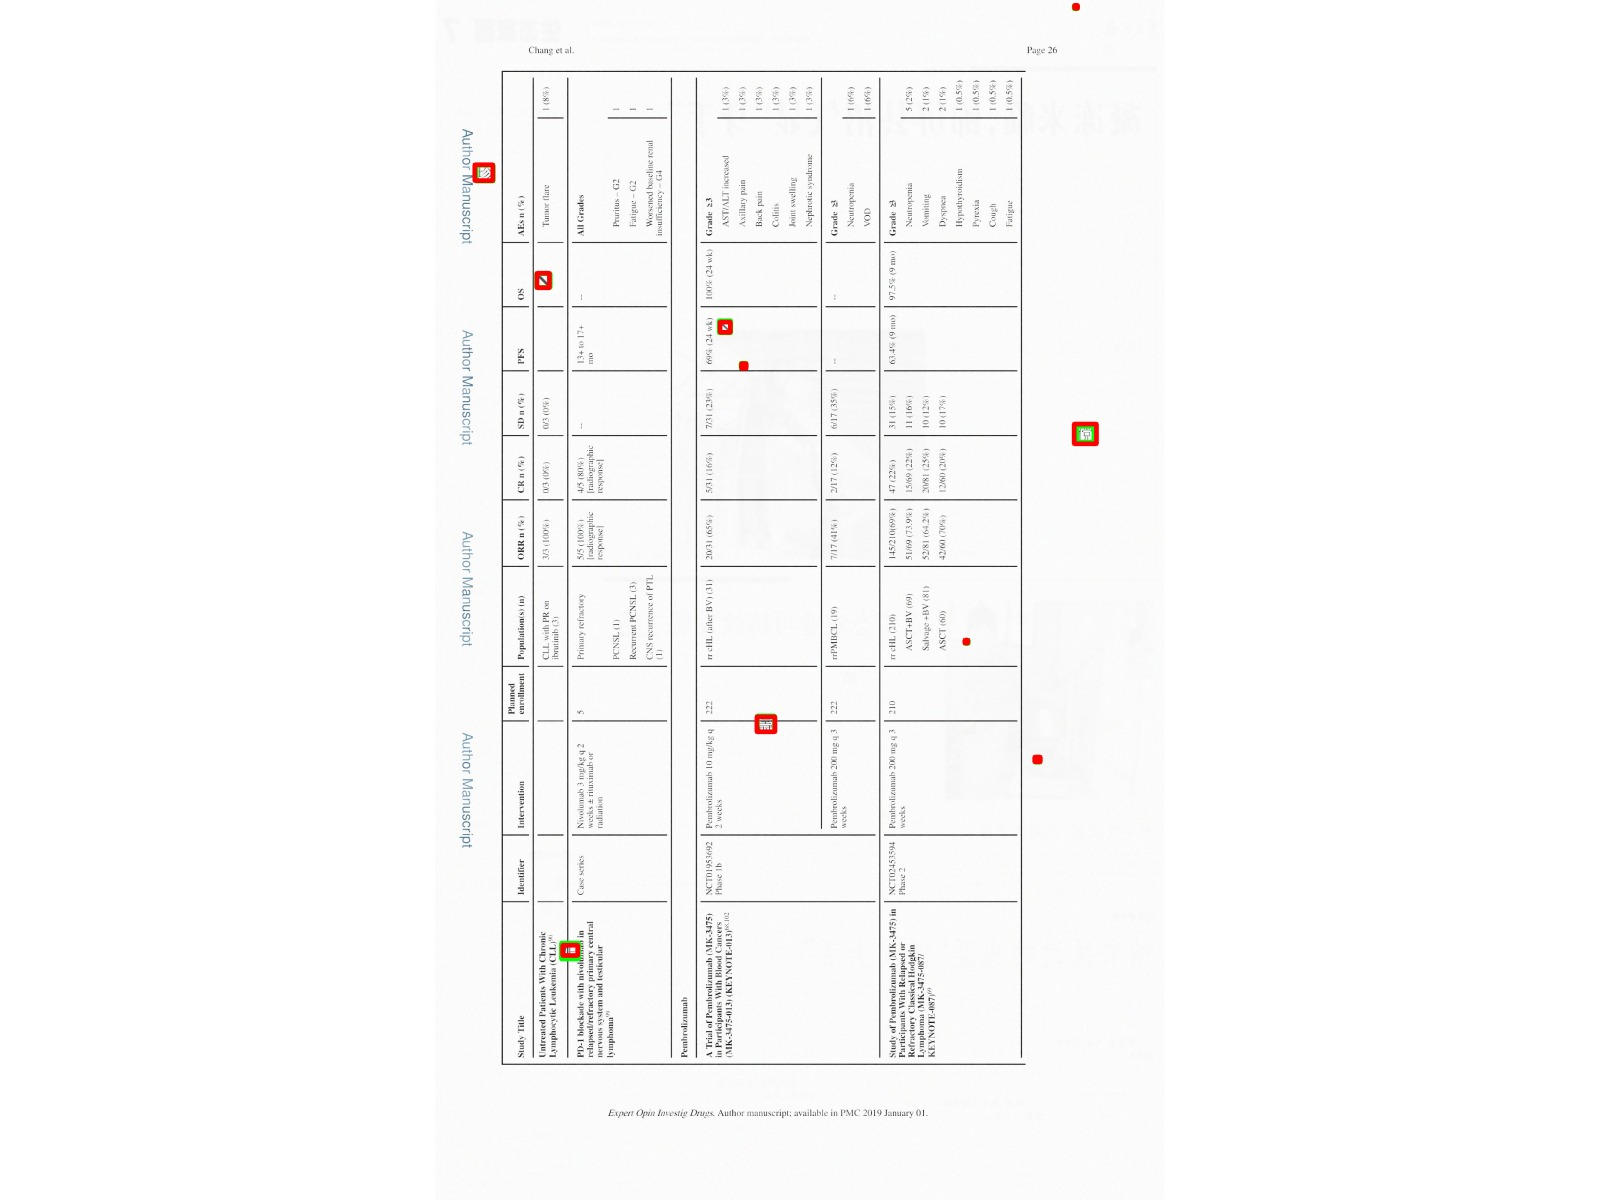
\includegraphics[width=\linewidth]{task1_qual_tp.png}\\[-1pt]
{\small (a) Correct detections}
\end{minipage}\hfill
\begin{minipage}[t]{0.48\textwidth}\centering
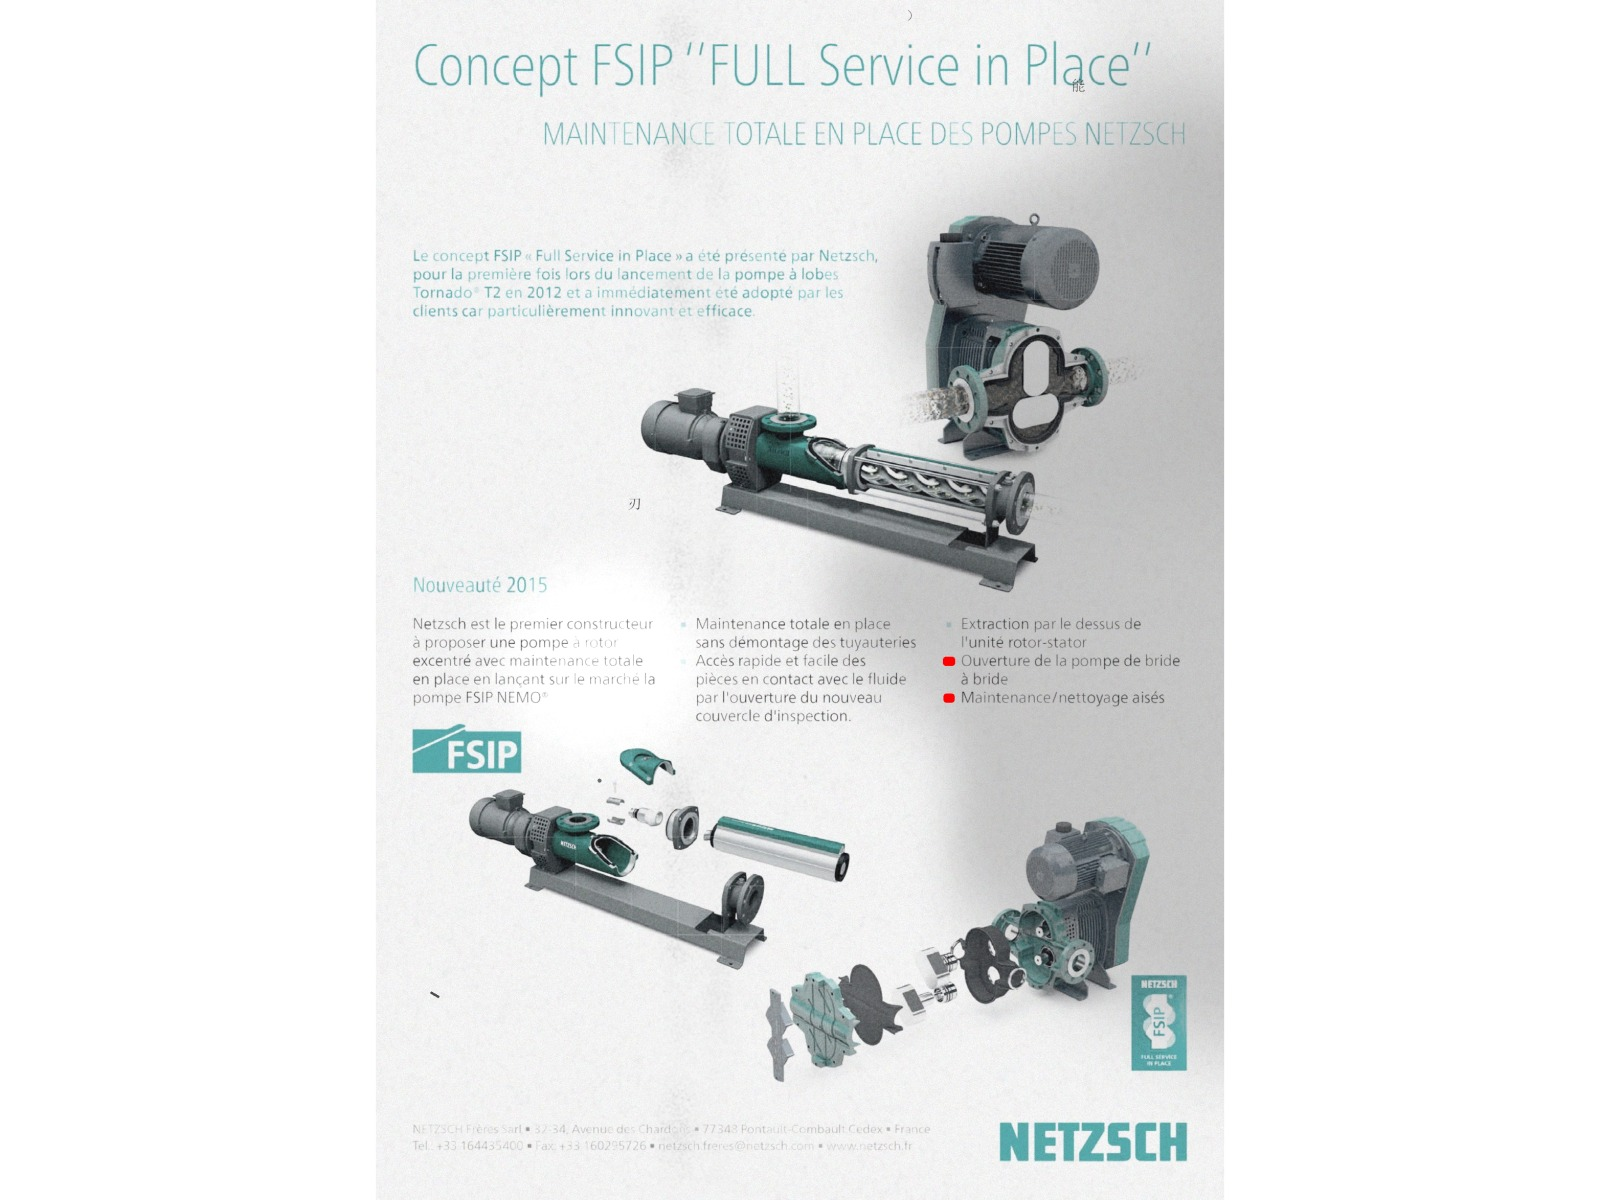
\includegraphics[width=\linewidth]{task1_qual_fp.png}\\[-1pt]
{\small (b) False positives}
\end{minipage}\\[6pt]
\begin{minipage}[t]{0.48\textwidth}\centering
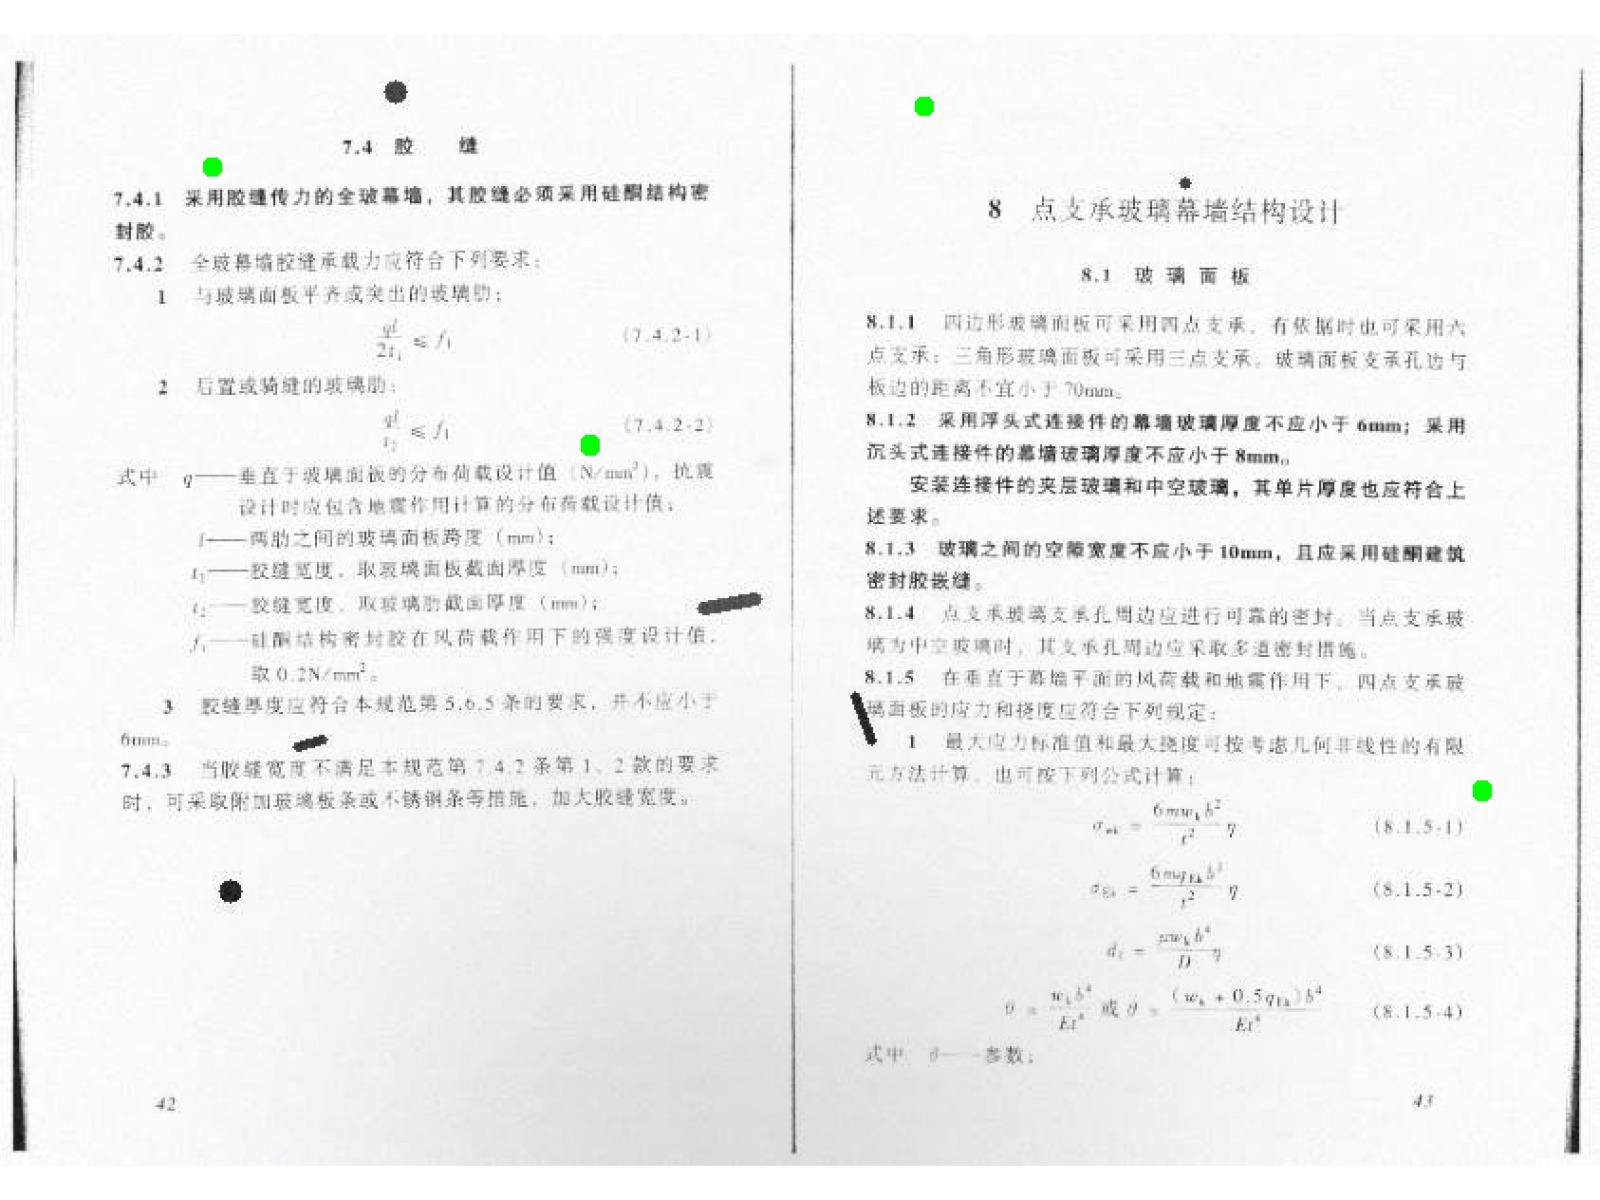
\includegraphics[width=\linewidth]{task1_qual_missed.png}\\[-1pt]
{\small (c) Missed boxes (never proposed)}
\end{minipage}\hfill
\begin{minipage}[t]{0.48\textwidth}\centering
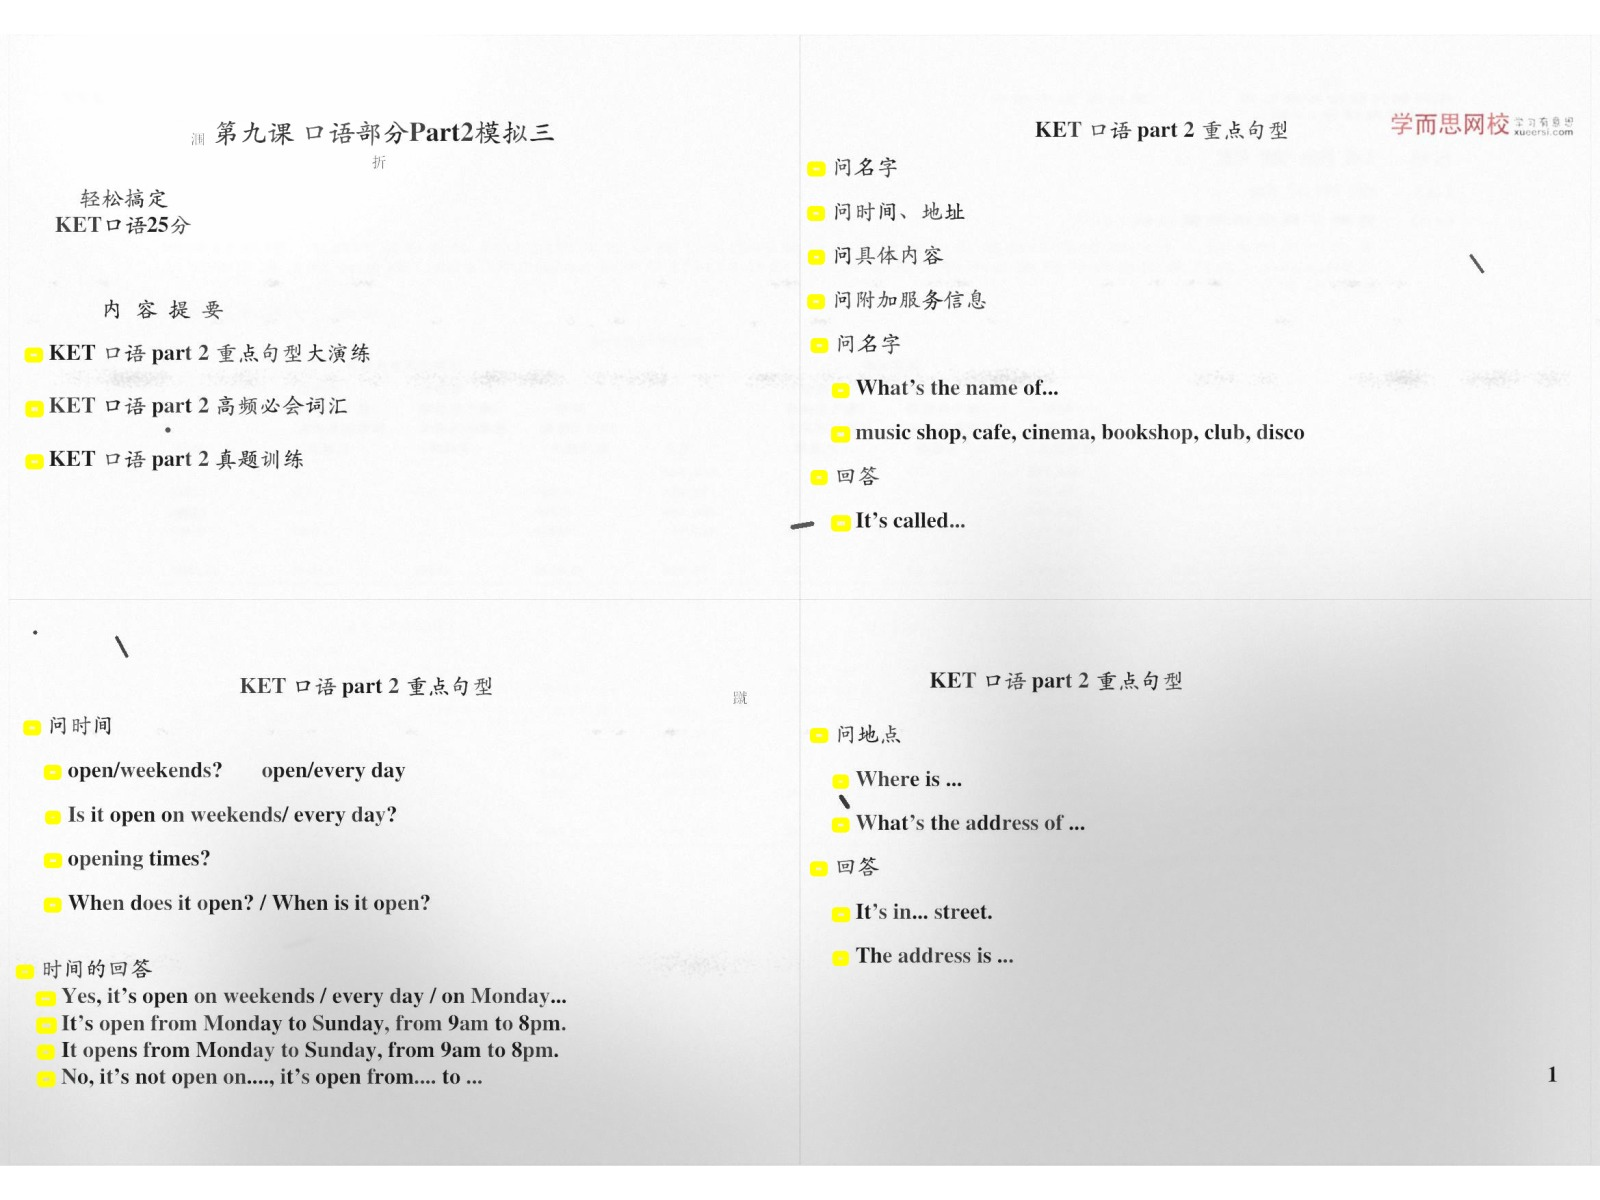
\includegraphics[width=\linewidth]{task1_qual_verifier.png}\\[-1pt]
{\small (d) Verifier corrections}
\end{minipage}
\caption{Task~1 qualitative results on out-of-fold predictions, with ground-truth and
predicted boxes overlaid on each pair.}
\label{fig:t1-qual}
\end{figure}

\noindent\textbf{Reachability of 0.97.} The final candidate set contains 1{,}352 of
the 1{,}407 boxes, so even a perfect rescorer caps at F1 0.9801 (Exp.~A15). The target
lies below this ceiling, but keeping all 1{,}352 matching proposals would still allow
at most about 28 false positives, against 50 out of fold, and the achieved 0.9465 is
0.0336 below the ceiling. Further gains need better proposals for the 55 boxes no
model finds, not better verifiers.

\noindent\textbf{Limitations.} Stride~2, the ink map, Siamese fusion, the polarity
filter, ink-map snapping and box-delta refinement were design choices that were not
ablated individually. Fold-0 comparisons rest on 268 boxes with no multi-seed noise
estimate. Exps.~A3 and~A4 were not repeated under the corrected fusion.

\section{Task 2: FRECA, Compliance Auditing with Grounded LLM Reasoning}
\label{sec:task2}

\subsection{Problem and Data}
\label{sec:t2-problem}

Given nine heterogeneous evidence files per farm export establishment (Registered
Establishment, RE), the system must audit compliance against 41 checking points (CPs)
drawn from the \emph{Export Control (Plants and Plant Products) Rules 2021}, emitting
\texttt{1} (compliant), \texttt{0} (non-compliant) or \texttt{N/A} per CP. Three hard
constraints govern the design: no hard-coded compliance logic anywhere in the pipeline,
LLM-API-only reasoning, and reproducibility.

The corpus has 99 raw folders that resolve to 100 logical cases, each with 7
\texttt{.docx} and 2 \texttt{.xlsx} tracks, and a 132-page policy document with 184
sections (Table~\ref{tab:t2-dataset} in Appendix~\ref{app:t2}). No labels were
provided; we hand-labelled a 10-case development set for internal measurement only,
and its labels were not independently verified. A median case is about 8.2K words
(22--26K tokens), so a whole case fits in one context window. Exploratory analysis
(Exp.~B1) found that one folder holds two complete establishments under the same RE
number (the ``missing'' 100th case), two folders lack the registration form, and some
apparent signals are generation noise.

\subsection{Submitted System}
\label{sec:t2-arch}

\begin{figure}[t]
\centering
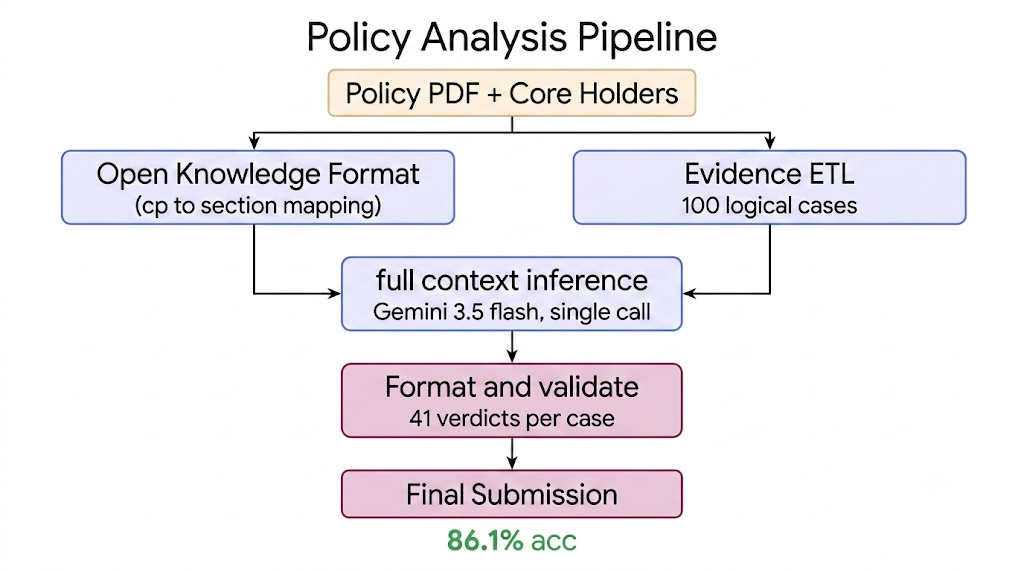
\includegraphics[width=0.52\textwidth]{task2_architecture.png}
\caption{Task~2 pipeline: an offline Open Knowledge Format (CP-to-section grounding)
and a per-case deterministic evidence ETL feed a single full-context call to
Gemini~3.5~Flash, followed by formatting and validation into the submission matrix.}
\label{fig:t2-arch}
\end{figure}

The pipeline (Fig.~\ref{fig:t2-arch}) has four phases.


\noindent\textbf{Phase 1: Open Knowledge Format (OKF), offline, once.} The policy PDF is chunked
into 184 sections by a deterministic regex on section headers. A one-time LLM pass
reads the statute text and maps each of the 41 CPs to its governing section(s),
producing a YAML-cited bundle of 18 unique sections (deduplicated from 64 citation
instances). It is stored with the system and can be re-derived on demand.

\noindent\textbf{Phase 2: deterministic evidence ETL, per case.} A canonical logical-case manifest
resolves the 99 folders into 100 cases by splitting the doubled folder;
an ingestion step flattens \texttt{.docx}/\texttt{.xlsx} files into track-tagged
markdown, preserving table structure, tolerating missing tracks and sorting
lexicographically for reproducibility. This layer contains no compliance logic.

\noindent\textbf{Phase 3: full-context inference, per case.} One prompt per case
($\sim$44K tokens) holds the complete evidence, the OKF bundle (CP texts and governing
sections) and a persona prompt enforcing identity anchoring, boilerplate-versus-signal
discipline and \texttt{N/A} discipline. Model: Gemini~3.5~Flash~\cite{geminiteam2023},
temperature 0, reasoning enabled; temperature~0 does not guarantee identical outputs
across runs. Output: structured JSON with 41 verdicts, reasoning and confidence.
% TODO: give the exact model string / snapshot ID used for the 100-case run

\noindent\textbf{Phase 4: formatting and validation.} Verdicts are enum-validated into the
submission matrix (RE Number~+~CP1\ldots CP41).

The ETL performs pure extraction and the CP-to-section mapping is LLM-derived from the
statute, so neither contains compliance rules. The persona prompt, however, carries a
CP38-motivated instruction added after Exp.~B9. We distinguish encoding a checking
point's \emph{requirement} (what the governing text obliges) from hard-coding the
\emph{expected answer} (instructing which verdict to emit for a specific evidence
string); the former is legitimate grounding, the latter is non-compliant. The added
wording is general in form --- ``where a register row has both a fixed target and a
case-specific status/verification note, the status note is the signal, not the
target'' --- but its examples name the concrete strings ``2-year retention verified''
and ``migration in progress'' / ``pending'' that separate compliant from
non-compliant rows in this dataset. It is therefore a general interpretation rule
with CP38-answer-specific examples, so the no-hard-coding constraint holds only
partially. The intervention was developed and scored on the same ten dev cases and
was never evaluated on unseen cases, so we do not claim the constraint is fully
satisfied.

\noindent\textbf{Production run} (Exp.~B14). With a 240-second per-call timeout and
per-case checkpointing, all 100 cases completed with no blanks and no parse failures,
using 4{,}493{,}869 tokens ($\sim$44.9K per case); the run was resumed four times after
key changes and credit or rate-limit stops without losing progress. The output holds
3{,}118 \texttt{1}, 982 \texttt{0} (23.95\%, against 17.6\% in the dev gold) and no
\texttt{N/A}. The 100th case, the second establishment in the doubled folder, was submitted under a
provisional ID.

\subsection{Development Path}
\label{sec:t2-experiments}


\noindent\textbf{Model choice.} With identical prompts, grounding and evidence
(Exp.~B4; Table~\ref{tab:t2-bakeoff} in Appendix~\ref{app:t2}), Gemini~3.5~Flash
reached 86.1\% against 76.6\% for Nemotron Ultra and 81.5\% for DeepSeek~V4~Pro.
Sonnet~5 scored highest (91.0\%) but was withdrawn
because the submission had to be reproducible through the team's own API key (an
access constraint, not a quality judgement); Gemini~3.5~Flash was the best model that
met it.

\noindent\textbf{Full context beat retrieval.} A hybrid RAG
branch~\cite{lewis2020rag} (BM25~\cite{robertson2009bm25} and bge-small dense
retrieval~\cite{xiao2024bge}, weighted fusion, ColBERT~\cite{khattab2020colbert}
rerank) scored 74.9\% at 610K tokens against 86.1\% at 442K for full context
(Exp.~B6). When a case fits in one
context window, retrieval only adds the risk of missing a decisive sentence: the
``maintained in Mandarin'' sentence was retrieved only $\sim$56\% of the time.

\noindent\textbf{Fewer calls.} The call architecture went from per-element,
per-persona calls (13 per case, megabyte-scale prompts) to a 3-persona ensemble
(3 calls, $\sim$215K tokens, with a hard-coded majority threshold) to the single
full-context call ($\sim$44K tokens) (Exp.~B8). On one case a Haiku persona ensemble
scored 70.7\% against 92.7\% for a single Sonnet pass at lower token cost (Exp.~B5);
this confounds model tier with ensembling, and we did not test a strong-model ensemble.

\noindent\textbf{Boilerplate versus signal.} CP38 (record retention) was being decided
from a date-range string that is byte-identical across compliant and non-compliant
cases. Telling the model that the per-case status note is the signal took CP38 from
4/10 to 10/10 on the in-sample dev set. This was measured on the Sonnet~5 development
run, \emph{not} on the submitted Gemini~3.5~Flash model, so it is a prompt-development
observation rather than a result of the submitted system; the same class of fix is
still needed for CP37 (Exp.~B10).

\noindent\textbf{Error analysis} on the dev set (Exps.~B10--B13): the model never emits
\texttt{N/A} (all 8 gold-\texttt{N/A} cells were predicted \texttt{1}), Element-4
(traceability) is weakest at 77.7\%, and CP39's gold is internally inconsistent.

\subsection{Results}
\label{sec:t2-results}

The organisers scored the submission at accuracy 0.7818, precision 0.7758, recall
0.7818 and F$_\beta$ 0.7783. Recall equal to accuracy indicates support-weighted
averaging. The 0.861 figure is \emph{in-sample development accuracy} on a 10-case
set that we self-labelled and then used to tune the prompts (including the CP38
wording); it is not an estimate of generalization, and we do not report it as such.
The official accuracy is 7.9 points below that in-sample number and below the worst
dev case (dev cases range from 80.5\% to 95.1\%; Exp.~B11), so the gap is not sampling
noise within the dev set. However, because no independent labelled evaluation set
exists, the cause of the official-score gap \emph{cannot be established from the
available evidence}; the following are hypotheses only: the dev labels are
self-assigned and unverified; the CP38 prompt was tuned on the dev set; CP39's gold
is inconsistent; and $n=10$. Over-flagging is a further hypothesis, since the
production run predicts \texttt{0} more often than the dev gold and class-0 precision
on the dev set was only 0.616.

\noindent\textbf{Limitations.} The ten dev cases are self-labelled and were used to
tune prompts, so dev accuracy is not held-out accuracy; the CP37--39 analysis used the
Sonnet run rather than the submitted model; the OKF was not ablated, and only 12 of 41
CPs were mapped identically by two mapping models; ensembling was not tested with a
strong base model; and the exact model snapshot is not recorded
(Appendix~\ref{sec:t2-limits}).

\section{Task 3: Real-Time Communication Flow Classification}
\label{sec:task3}

\subsection{Problem and Data}
\label{sec:t3-problem}

Given only the first five packets of a real-time communication (RTC) flow (packet
lengths and relative timestamps), the system must predict which of five applications
(Discord, Google Meet, Messenger, WhatsApp, Zoom) produced the flow and whether it is a
voice or a video call, giving ten classes. The organisers report accuracy, precision,
recall and F$_\beta$; for our submission recall equals accuracy, which points to
support-weighted averaging. During development we optimised macro-F1, which weights
the small classes (40 Google Meet voice flows) as much as the large ones (256 Discord
video flows).

There are 1{,}285 training and 327 test flows (Table~\ref{tab:t3-data} in
Appendix~\ref{app:t3}), and train and test are exchangeable (adversarial-validation
AUC 0.529; Exp.~C1). Three properties dominate the design space: no call identifier is
released although flows from the same call are near-duplicates (an estimated
$\approx$400 source calls); more than half of all flows (56.5\%) have a window in which
every packet is below 300 bytes, i.e.\ only audio-sized packets whatever the call
mode; and the dataset is small.

\subsection{Submitted System}
\label{sec:t3-arch}

\begin{figure}[t]
\centering
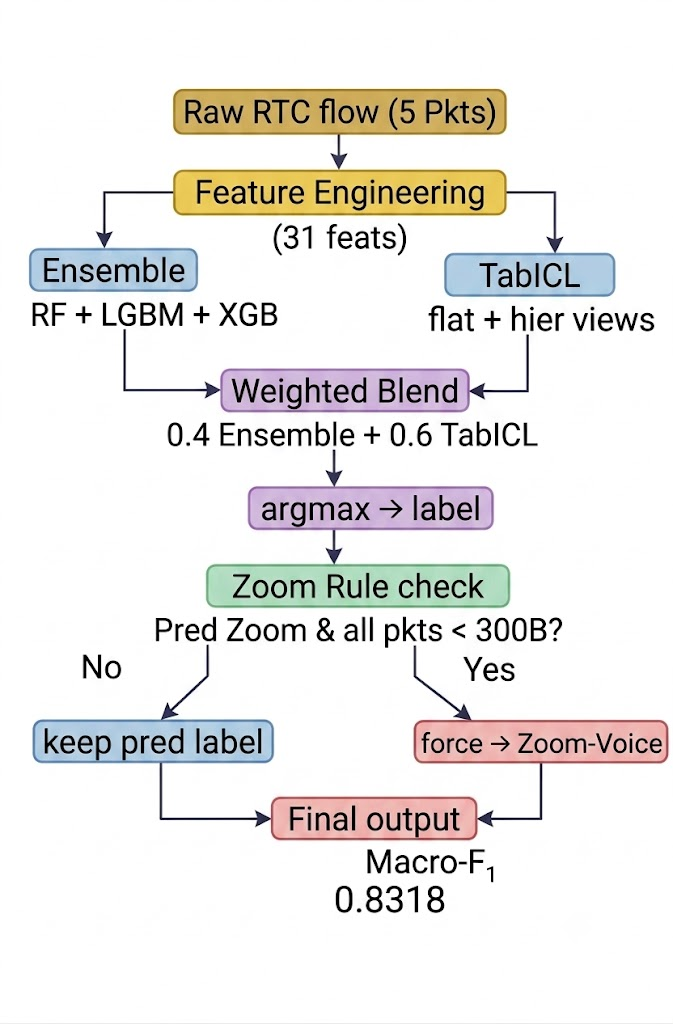
\includegraphics[width=0.36\textwidth]{task3_architecture.png}
\caption{Task~3 pipeline: 31 columns feed the tree ensemble (Branch~A) and 241
columns feed TabICL in flat and hierarchical views (Branch~B); the probabilities are
blended $0.4/0.6$, and a parameter-free rule sends audio-only Zoom windows to
Zoom\_voice.}
\label{fig:t3-arch}
\end{figure}

The pipeline (Fig.~\ref{fig:t3-arch}) has five stages and two feature
representations.


\noindent\textbf{Stage 0: features.} Branch~A uses 31 compact columns: five lengths, four
timestamps, four length differences, four inter-arrival gaps, the lengths in rank
order, argmax/argmin position, range, mean, standard deviation, median and total span,
plus the logarithm of the fourth packet length and the position of the largest
packet-to-packet size increase. Branch~B uses 241 deterministic columns (raw and log
values, inter-arrival and length statistics, sequence shape, protocol bands and
residues, burst structure, rate and spectral terms). No feature depends on labels.

\noindent\textbf{Stage 1: Branch A, tree ensemble.} RandomForest~\cite{breiman2001rf} (600 trees,
balanced-subsample weights), LightGBM~\cite{ke2017lightgbm} (400 trees, depth 4, 15
leaves, learning rate 0.05, balanced) and XGBoost~\cite{chen2016xgboost} (400 trees,
depth 4, learning rate 0.05, subsample and column sample 0.8). Probabilities are
averaged with equal weight, softened by a temperature $T=2$
($\tilde p_k\propto\bar p_k^{1/T}$), divided by the empirical class prior
$\hat\pi_k$ and renormalised. All estimators run single-threaded (Exp.~C9).

\noindent\textbf{Stage 2: Branch B, TabICL.} TabICL~\cite{qu2025tabicl} with 16 internal
estimators and no tuning, in a flat ten-class view and a hierarchical view (an
application head and per-application voice/video heads); the two probability vectors
are averaged.
% TODO: confirm the hierarchical view is the product P(app)*P(mode|app)

\noindent\textbf{Stage 3: blend.} $p=0.4\,p_{\mathrm{A}}+0.6\,p_{\mathrm{B}}$, then argmax. The
weight is the median of ten weights, each chosen on the training side of one grouped
fold (Exp.~C23).

\noindent\textbf{Stage 4: Zoom rule.} If the blended label is either Zoom class and all five
packet lengths are below 300 bytes, the label is set to Zoom\_voice. The rule has no
fitted parameter (Exps.~C18--C19).

\noindent\textbf{Validation protocol.} Every Branch~B selection decision is scored on
grouped folds (\texttt{StratifiedGroupKFold}, 5 splits $\times$ 2 repeats) over a
pseudo-call key, the packet-length tuple rounded to 8 bytes joined with the rounded
log-duration, which yields 1{,}107 pseudo-groups. Negative controls pass (shuffled
labels 0.1549, prior-only 0.1992; Exp.~C2). Only nested values of fitted quantities (blend
weight, offsets, biases) are used for choosing. Branch~A, developed earlier under
stratified folds, is the one exception. Unlabelled test flows are never used to fit a
label-dependent quantity.

\noindent\textbf{Submission} (Exp.~C25). Branch~A was refit on all 1{,}285 rows
\emph{without} the per-class offsets and specialist of Exp.~C7, so that the blend
receives corrected probabilities rather than outputs shifted toward recall; Branch~B
test probabilities come from a full-data refit. The rule routed 43 of the 327 test
flows to Zoom\_voice, in line with the training proportion.

\subsection{Development Path}
\label{sec:t3-experiments}

\noindent\textbf{Model search.} 2{,}377 grid points over eleven model families, followed
by Optuna~\cite{optuna}, put boosted trees ahead; distance, kernel, linear and neural
models trailed by 9--11 points (Exp.~C3). TabICL with no tuning beat the best searched
point (LightGBM, 0.8249) at every feature width, though the paired difference is not
significant (66 rows won against 49, $p=0.135$; Exp.~C10). Feature pruning,
label-aware features, pretraining on a public corpus~\cite{mirage}, probe features, a
tuple lookup and call-level aggregation did not help (Exps.~C4, C12, C13, C15).

\noindent\textbf{One pair bounds the score.} The standing tree configuration made 237
errors, 175 of them in audio-only windows and 68 between Zoom\_voice and Zoom\_video
alone (Exp.~C17). Inside audio-only windows the Zoom pair is not separable: the subset
is exactly balanced (80 voice, 80 video) and the grouped AUC of video against voice is
0.551, against 0.83--0.88 for the other applications (Exp.~C18). Even with every other
flow correct, accuracy is capped at 0.9377 and macro-F1 at 0.9364.

\noindent\textbf{A derived rule, not a fitted one.} On an evenly split, inseparable
subset every assignment has the same accuracy but not the same macro-F1: sending all
160 flows to Zoom\_voice gives F1 0.667 (voice) and 0.697 (video), against 0 and 0.811
for Zoom\_video (Exp.~C19). The rule improved macro-F1 for all six model families in
every view (Exp.~C20), whereas fitted per-class biases gained in sample and lost nested
(Exps.~C14, C21). It is neutral for accuracy (0.8233 $\rightarrow$ 0.8241).

\noindent\textbf{Two branches.} Branch~A's complementary strength is Zoom\_voice
recall (0.712 against 0.438 for Branch~B; Exp.~C22). Nested selection picked blend weights from 0.25 to 0.55 across
folds, median 0.40 (Exp.~C23). The blend improves on Branch~B with the rule by
$+0.0039$ to $+0.0072$ macro-F1, but the bootstrap interval includes zero (Exp.~C24).

\subsection{Results}
\label{sec:t3-results}

The organisers scored the submission at accuracy 0.8746, precision 0.9211, recall
0.8746 and F$_\beta$ 0.883 on the 327 test flows. Because the official metrics are
support-weighted, F$_\beta$ is not comparable with our macro-F1 estimates in
Table~\ref{tab:t3-summary}. The test accuracy is 3.6 points above the cross-validated
accuracy of the blend (0.8389); with $n=327$ the standard error of an accuracy near
0.87 is about 1.9 points, so the difference is about two standard errors. Possible
contributors are training on all 1{,}285 flows rather than four fifths and the
weighted metric favouring large classes; we did not test either.

\begin{table}[t]
\caption{Task~3 results. Cross-validation rows are pooled grouped out-of-fold
predictions (each of the 1{,}285 rows scored twice); the first two rows are single-model
references (Exps.~C3, C10).}
\label{tab:t3-summary}
\centering
\small
\begin{tabular}{lccc}
\toprule
Configuration & Accuracy & Macro-F1 & Fold mean \\
\midrule
Official test (weighted metrics, $n=327$) & \textbf{0.8746} & --- & --- \\
\midrule
Best searched point, LightGBM (C3) & 0.8249 & 0.8069 & --- \\
TabICL, default, 241 columns (C10) & 0.8389 & 0.8232 & --- \\
Branch A, corrected probabilities (stratified folds) & 0.7961 & 0.7900 & --- \\
Branch B, flat+hier average & 0.8358 & 0.8201 & 0.8175 \\
Branch B + Zoom rule & 0.8342 & 0.8292 & 0.8268 \\
Blend, nested weight, no rule & 0.8389 & 0.8319 & 0.8286 \\
Blend, nested weight, + Zoom rule (submitted) & --- & 0.8345 & \textbf{0.8318} \\
Blend, $w=0.40$, + Zoom rule$^{a}$ & 0.8389 & 0.8366 & --- \\
\midrule
\multicolumn{4}{l}{\footnotesize $^{a}$ $w$ located on the same rows (Exp.~C23); optimistic.}\\
\bottomrule
\end{tabular}
\end{table}

\noindent\textbf{Limitations.} Branch~A's out-of-fold probabilities come from
stratified rather than grouped folds, so the 0.40 weight on Branch~A is, if anything,
too high and the nested estimate of 0.8318 is likely somewhat optimistic. The Branch~B
variant, the 16-estimator setting and the blend were chosen among near-equal
candidates on the same 1{,}285 rows. The Zoom rule is a property of this dataset's Zoom
audio-only windows and is not claimed to transfer (Appendix~\ref{sec:t3-limits}).

\section{Cross-Task Discussion}
\label{sec:discussion}

\noindent\textbf{Development estimates and official scores disagreed, in both
directions.} Task~1's pooled out-of-fold F1 of 0.9465 became 0.9577 officially and
Task~3's cross-validated accuracy of 0.8389 became 0.8746, while Task~2's dev accuracy
of 0.861 became 0.7818, outside the spread of its own dev cases. In Tasks~2 and~3 official recall equals accuracy, so the
metric is support-weighted, and our macro-averaged concerns (Task~2) and macro-F1
objective (Task~3's rule, neutral on accuracy) did not transfer.

\noindent\textbf{Secondary diagnostics show where the headline metric is bounded.} The
Task~1 recall ceiling (0.9801) lies 0.0336 above the out-of-fold F1 (Exps.~A8, A15);
Task~2's per-class and per-element breakdowns exposed the missing \texttt{N/A} class
and the weak traceability element (Exps.~B12, B13); and one inseparable class pair caps
Task~3's macro-F1 at 0.9364 (Exp.~C18).

\noindent\textbf{Negative results need a bug hypothesis first.} Task~1's verifier
looked like a dead end ($+0.0009$, Exp.~A10) until it was retrained on raw candidates
and gained on all five folds (Exp.~A11), and fusion bugs had made TTA and ensembling
look harmful (Exps.~A16, A17). Data structure is likewise an engineering problem and a
leakage risk: fold-scoped synthesis (Task~1), a logical-case manifest (Task~2,
Exp.~B1) and pseudo-call groups (Task~3, 1{,}107 groups against an estimated 400 calls,
so grouped cross-validation may still leak).
The practical lesson is to state next to every number which protocol produced it,
and to treat the organisers' held-out scores as the only reliable estimate.


\section{Conclusion}
\label{sec:conclusion}

Officially, Task~1 scored \textbf{0.9577} (out-of-fold 0.9465; candidate-set ceiling
0.9801), Task~2 scored \textbf{0.7818} with a single full-context LLM call (development
estimate 0.861), and Task~3 scored \textbf{0.8746} accuracy with gradient-boosted
trees, TabICL and a deterministic rule (pooled grouped out-of-fold accuracy 0.8389). The common
lessons were to separate model quality from decoding and scoring effects, to measure
what the headline metric hides, and to suspect the experiment before the idea when a
result is unexpectedly negative.

\begin{credits}

\subsubsection{Compute}
Task~1 detectors and verifiers were trained on A100 GPUs on Modal.

\subsubsection{Use of large language models}
Gemini~3.5~Flash is the reasoning component of the Task~2 system. Claude Sonnet~5 was used in the Task~2 development bake-off and per-checking-point analysis (Exps.~B4, B9, B10) but not in the submitted system. Claude was used to restructure and copy-edit this manuscript; the authors checked all content.

\subsubsection{\ackname}
We thank the CyberAI Cup 2026 organisers for providing the datasets and evaluation infrastructure used in this work.

\subsubsection{\discintname}
The authors have no competing interests to declare that are relevant to the content of this article.

\end{credits}

\begin{thebibliography}{21}

\bibitem{zhou2019centernet}
Zhou, X., Wang, D., Kr{\"a}henb{\"u}hl, P.: Objects as points. arXiv preprint arXiv:1904.07850 (2019)

\bibitem{liu2022convnext}
Liu, Z., Mao, H., Wu, C.-Y., Feichtenhofer, C., Darrell, T., Xie, S.: A ConvNet for the 2020s. In: Proceedings of the IEEE/CVF Conference on Computer Vision and Pattern Recognition (CVPR), pp. 11976--11986 (2022)

\bibitem{he2016resnet}
He, K., Zhang, X., Ren, S., Sun, J.: Deep residual learning for image recognition. In: Proceedings of the IEEE Conference on Computer Vision and Pattern Recognition (CVPR), pp. 770--778 (2016)

\bibitem{ronneberger2015unet}
Ronneberger, O., Fischer, P., Brox, T.: U-Net: convolutional networks for biomedical image segmentation. In: MICCAI 2015, LNCS, vol.~9351, pp. 234--241. Springer, Cham (2015)

\bibitem{solovyev2021wbf}
Solovyev, R., Wang, W., Gabruseva, T.: Weighted boxes fusion: ensembling boxes from different object detection models. Image and Vision Computing \textbf{107}, 104117 (2021)

\bibitem{breiman2001rf}
Breiman, L.: Random forests. Machine Learning \textbf{45}(1), 5--32 (2001)

\bibitem{chen2016xgboost}
Chen, T., Guestrin, C.: XGBoost: a scalable tree boosting system. In: Proceedings of the 22nd ACM SIGKDD International Conference on Knowledge Discovery and Data Mining, pp. 785--794 (2016)

\bibitem{ke2017lightgbm}
Ke, G., Meng, Q., Finley, T., Wang, T., Chen, W., Ma, W., Ye, Q., Liu, T.-Y.: LightGBM: a highly efficient gradient boosting decision tree. In: Advances in Neural Information Processing Systems 30 (NeurIPS), pp. 3146--3154 (2017)

\bibitem{qu2025tabicl}
Qu, J., Holzm{\"u}ller, D., Varoquaux, G., Le Morvan, M.: TabICL: a tabular foundation model for in-context learning on large data. In: Proceedings of the 42nd International Conference on Machine Learning (ICML). PMLR (2025)

\bibitem{robertson2009bm25}
Robertson, S., Zaragoza, H.: The probabilistic relevance framework: BM25 and beyond. Foundations and Trends in Information Retrieval \textbf{3}(4), 333--389 (2009)

\bibitem{lewis2020rag}
Lewis, P., Perez, E., Piktus, A., Petroni, F., Karpukhin, V., Goyal, N., K{\"u}ttler, H., Lewis, M., Yih, W.-t., Rockt{\"a}schel, T., Riedel, S., Kiela, D.: Retrieval-augmented generation for knowledge-intensive NLP tasks. In: Advances in Neural Information Processing Systems 33 (NeurIPS), pp. 9459--9474 (2020)

\bibitem{khattab2020colbert}
Khattab, O., Zaharia, M.: ColBERT: efficient and effective passage search via contextualized late interaction over BERT. In: Proceedings of the 43rd International ACM SIGIR Conference on Research and Development in Information Retrieval, pp. 39--48 (2020)

\bibitem{xiao2024bge}
Xiao, S., Liu, Z., Zhang, P., Muennighoff, N., Lian, D., Nie, J.-Y.: C-Pack: packed resources for general Chinese embeddings. In: Proceedings of the 47th International ACM SIGIR Conference on Research and Development in Information Retrieval, pp. 641--649 (2024)

\bibitem{geminiteam2023}
Google DeepMind: Gemini~3.5~Flash model card. Accessed via the alias \texttt{google/gemini-3.5-flash}, August 2026

\bibitem{optuna} Akiba, T., Sano, S., Yanase, T., Ohta, T., Koyama, M.: Optuna: a next-generation hyperparameter optimization framework. In: Proceedings of the 25th ACM SIGKDD International Conference on Knowledge Discovery and Data Mining, pp. 2623--2631 (2019)
\bibitem{catboost} Prokhorenkova, L., Gusev, G., Vorobev, A., Dorogush, A.V., Gulin, A.: CatBoost: unbiased boosting with categorical features. In: NeurIPS 31 (2018)
\bibitem{mcnemar} McNemar, Q.: Note on the sampling error of the difference between correlated proportions or percentages. Psychometrika 12(2), 153--157 (1947)
\bibitem{tabpfn} Hollmann, N., et al.: Accurate predictions on small data with a tabular foundation model. Nature 637, 319--326 (2025)
\bibitem{guo} Guo, C., Pleiss, G., Sun, Y., Weinberger, K.Q.: On calibration of modern neural networks. In: Proceedings of the 34th International Conference on Machine Learning (ICML), pp. 1321--1330 (2017)
\bibitem{kull} Kull, M., et al.: Beyond temperature scaling: obtaining well-calibrated multiclass probabilities with Dirichlet calibration. In: NeurIPS 32 (2019)
\bibitem{mirage} Guarino, I., et al.:MIRAGE-App$\times$Act-2024: A novel dataset for mobile app and activity traffic analysis. In: WiMob 2024 (2024)
\end{thebibliography}

\clearpage
\appendix
\section{Task 1: Dataset, Full Experimental Log and Bugs}
\label{app:t1}
\renewcommand{\expprefix}{A}

\subsection{Dataset and Data Usage}

Table~\ref{tab:t1-dataset} gives the full dataset statistics. The change-polarity
labels (842 additions, 558 modifications, zero pure deletions) sum to 1{,}400 of the
1{,}407 boxes.
% TODO: explain the 7 boxes with no polarity label from the polarity script
The unlabelled test templates were used as a source for synthetic training pairs
(Experiment~5). No test-set labels exist to us, and no test photographs were used for
threshold selection.
% TODO: confirm that only templates, not test photographs, entered synthesis

\begin{table}[h]
\caption{Task 1 dataset statistics.}\label{tab:t1-dataset}
\centering
\small
\begin{tabular}{lp{6.2cm}}
\toprule
Quantity & Value \\
\midrule
Train pairs / boxes & 200 / 1{,}407 \\
Test pairs & 100 \\
Dataset size & 2.5\,GB \\
Boxes per image & 3--11, median 7 \\
Median box size & $22\times22$\,px \\
Boxes under $16\times16$\,px (both sides) & 419 \\
Boxes exactly $8\times8$\,px & 83 \\
Change polarity & 842 additions, 558 modifications, 0 deletions (7 boxes unlabelled) \\
Alignment & no warp needed for 284/300 pairs, p95 residual $\leq0.26$\,px \\
Photo degradation & 2--6$\times$ lower Laplacian variance than template; $\sim$18\% heavy shadow \\
\bottomrule
\end{tabular}
\end{table}

\subsection{Development Path Summary}

Table~\ref{tab:t1-path} summarises the steps from the first baseline to the pooled
five-fold result (Section~\ref{sec:t1-experiments}).

\begin{table}[h]
\caption{Task~1 development path. Fold-0 out-of-fold F1 (268 boxes; one box
$=0.004$ F1) unless marked as pooled over five folds (1{,}407 boxes).}
\label{tab:t1-path}
\centering
\small
\begin{tabular}{llcl}
\toprule
Step & Exp. & F1 & Note \\
\midrule
Classical normalised difference & A1 & 0.0293 & recall 0.572, precision 0.015 \\
Siamese CenterNet, single model & A2 & 0.9049 & reference control \\
\texttt{\_aug} weights, old $\rightarrow$ new decode & A6 & 0.9257 & same weights, $+0.021$ \\
$+$\,\texttt{\_augsyn} detector (WBF ensemble) & A9 & 0.9266 & ceiling $0.944\rightarrow0.963$ \\
$+$\,cross-fold verifier & A11 & 0.9430 & gain on all five folds \\
Pooled, detector only & A13 & 0.9385 & nested threshold: 0.9385 \\
Pooled, detector $+$ verifier & A12 & 0.9465 & nested threshold: 0.9435 \\
\bottomrule
\end{tabular}
\end{table}

\subsection{Organisation of the Log}

Nineteen experiments were numbered in sequence; we group them by theme below. Experiments~6 and~7 are the same study and are reported together as Experiment~6 (the number~7 is unused); Experiment~19, an infrastructure failure with no effect on any result, is described in Appendix~\ref{app:t1-detach}. Within this appendix, ``Experiment~$n$'' refers to Experiment~A$n$. Unless noted, results are reported on fold~0 out-of-fold validation before the full 5-fold run (Experiment~12). Numbers in Experiments~6 and later were produced after the fusion bug of Experiment~16 was fixed; Experiments~3 and~4 were not repeated (see the limitations in Section~\ref{sec:t1-results}).

\subsection{Baseline establishment}

\begin{explog}{1}{Classical normalized-difference baseline}
\item[Hypothesis] A naive pixel-wise difference between template and photo can localize content changes directly, since differences should stand out after alignment.
\item[Method] Compute normalized pixel difference between aligned template and photo, threshold to get blobs, convert blobs to boxes.
\item[Result] Recall 0.572 at precision 0.015. Global F1 $=0.0293$.
\item[Inference] Fails catastrophically because every glyph edge fires --- the photo is systematically softer/blurrier than the template, so raw differencing cannot distinguish scan/print noise from genuine changes. Precision, not recall, is the hard part of this task. Blur-matching template to photo before differencing is a prerequisite, not an optimization.
\item[Verdict] Rejected as a primary approach; directly informed the design of the Stage~0 ink-map preprocessing.
\end{explog}


\begin{explog}{2}{Siamese CenterNet, single model, fold 0 (reference baseline)}
\item[Hypothesis] A shared-weight ConvNeXt-tiny Siamese encoder over 4-channel (BGR~+~ink) streams, decoded through a U-Net path to output stride~2 (instead of the standard stride~4), can localize the small (median $22\times22$, many $8\times8$) ground-truth boxes at sub-pixel precision.
\item[Method] Train a Siamese CenterNet with four heads (centre heatmap, w/h, sub-pixel offset, auxiliary change mask) on $768$\,px tiles, 60\% sampled around annotated differences. Decode at \texttt{score\_thr}$=0.05$, \texttt{max\_boxes}$=40$, no TTA.
\item[Result] Fold~0 OOF: F1 $=0.9049$, Precision $=0.922$, Recall $=0.888$ (TP 238 / FP 20 / FN 30 on 268 boxes).
\item[Inference] Establishes that stride-2 small-object detection is viable and sets the control number (0.9049) that every subsequent change is measured against.
\item[Verdict] Kept as the baseline architecture; became the reference for all fold-0 controlled experiments.
\end{explog}


\subsection{Detector-side ablations}

\begin{explog}{3}{Size-relative width/height loss}
\item[Hypothesis] Standard w/h regression loss is size-blind and should under-penalize errors on tiny ($8\times8$) boxes relative to large ones; a size-relative loss should improve small-box localization.
\item[Method] Replace absolute w/h loss with a size-normalized variant; train on fold~0 with identical settings otherwise.
\item[Result] Fold~0 finished at TP~238 / FP~20 / FN~30 --- exactly the reference's counts.
\item[Inference] No measurable effect. One box is worth 0.004 F1 on 268 validation boxes, and we estimate run-to-run noise at about $\pm0.02$ F1. Identical TP/FP/FN counts to the reference are unusual at that noise level, so they may mean that the flag did not take effect or that the log was copied from the baseline run.
\item[Verdict] Dropped; kept as an option, disabled by default.
% TODO: (1) verify in the Exp.3 log that the size-relative loss flag was active and the counts are not copied from Exp.2;
% TODO: (2) the +-0.02 noise estimate and the ``three runs in 0.890--0.905'' claim need a seeds table; add it or delete both.}
\end{explog}


\begin{explog}{4}{EMA weights (decay 0.999)}
\item[Hypothesis] Exponential moving average of weights should stabilize training and yield a better final checkpoint than raw weights.
\item[Method] Track an EMA of model weights during training; compare EMA versus raw weights at each checkpoint on fold~0 validation.
\item[Result] EMA weights were never selected over raw weights until the final two epochs, where they tied.
\item[Inference] No consistent benefit within the training budget used; on a short schedule EMA does not have time to average out enough noise to help.
\item[Verdict] Neutral; dropped as default, kept behind a flag.
\end{explog}


\begin{explog}{5}{Synthetic small-mark pairs}
\item[Hypothesis] The model under-detects sub-12\,px boxes because there are too few real examples; synthetically generating small-mark differences on real page layouts should raise coverage of that size band.
\item[Method] Generate synthetic template/photo pairs with invented small-mark edits on real page layouts, fold-scoped to avoid leakage (Section~\ref{sec:t1-arch}). Train a model variant (\texttt{\_augsyn}) on real~+~synthetic data.
\item[Result] Standalone F1 is \emph{worse} than the augmented-only model (0.896 vs.\ 0.926). But candidate recall ceiling (fraction of ground-truth boxes present anywhere in the candidate list at IoU~0.5) rose from 0.891 (\texttt{\_aug}, the matched control without synthetic data) to 0.922 on the sub-12\,px band specifically, and the overall ceiling rose from 0.9440 to 0.9590. (Comparing with the original model's 0.828 would also credit the dihedral augmentation, which \texttt{\_augsyn} shares with \texttt{\_aug}.)
\item[Inference] This model looks like a failure on F1 alone because it proposes very aggressively (10{,}238 candidates vs.\ 421 for the original, though these counts come from different decode settings and are not like-for-like), but it recovers boxes no other model ever proposes.
\item[Verdict] Kept, but only as an ensemble member, never standalone.
% TODO: recount candidates for both models at one decode setting
% TODO: Its value is in ensemble coverage, not standalone accuracy --- a fact that would have been missed without explicitly measuring the recall ceiling separately from F1.
\end{explog}


\subsection{Decode-time optimization and the model/decode entanglement}

\begin{explog}{6}{Decode settings and the model/decode interaction}
\item[Hypothesis] Flips and transposes are free label-preserving augmentation and should improve generalization; if it appears not to help, the measurement method (decode settings) should be suspected before the change itself. A low score threshold, a higher box cap and 8-view TTA should surface more true candidates, at the cost of noise that WBF and the verifier can filter.
\item[Method] Train with dihedral augmentation (\texttt{\_aug}); evaluate the \emph{same weights} first at the old reference decode (\texttt{score\_thr}$=0.05$, \texttt{max\_boxes}$=40$, no TTA), then at \texttt{score\_thr}$=0.02$, \texttt{max\_boxes}$=300$ with 8-view TTA fused by WBF~\cite{solovyev2021wbf}. Sweep threshold, box cap and view count on fold-0 out-of-fold predictions.
\item[Result] $0.9049$ at the old decode (looked worthless) versus $0.9257$ at the new decode: the same weights, $+0.021$ F1, about five boxes on 268.
\item[Inference] Because the weights are identical, training-seed noise does not enter this comparison; the remaining uncertainty is the validation sample. A paired bootstrap over images would give an interval; we did not run it. Every earlier ``no gain'' verdict on augmentation had been measured through a lossy decoder, so comparing models at a fixed default decode compares decoders as much as models. This was the most consequential methodological correction in the project.
\item[Verdict] Kept: augmentation is valuable but only visible once decode is fixed; \texttt{score\_thr}$=0.02$, \texttt{max\_boxes}$=300$, 8-view TTA with WBF became the standard decode.
% TODO: add the sweep table (score_thr x max_boxes x views -> F1); the old Exp.7 gave no numbers
% TODO: verify in the logs that 0.9049 here is a separate measurement and not the Exp.2 number reused}
\end{explog}

\subsection{Ensembling and recall-ceiling diagnostics}
\begin{explog}{8}{Recall ceiling measurement across model variants}
\item[Hypothesis] F1 alone cannot reveal whether a model's failures come from missing candidates (unrecoverable) or from mis-scored candidates (recoverable by rescoring); ceiling analysis will separate these.
\item[Method] For each model/combination, compute the fraction of ground-truth boxes present anywhere in the candidate list at IoU~0.5, regardless of score, on fold~0 with TTA at score~0.02. Compare against the sub-12\,px ceiling specifically.
\item[Result] Original: ceiling $0.9403$ (sub-12px $0.828$), F1 $0.9049$. \texttt{\_aug}: ceiling $0.9440$ ($0.891$), F1 $0.9257$. \texttt{\_augsyn}: ceiling $0.9590$ ($0.922$), F1 $0.8956$ (worse F1, much better ceiling). \texttt{\_aug}+\texttt{\_augsyn} combined: ceiling $0.9627$ ($0.9375$), F1 $0.9266$ (best two-model combo). A third model (\texttt{\_augpix}) is reported with ceiling $0.959$.
\item[Inference] Nothing downstream can recover a box that was never proposed, so the ceiling bounds every rescoring idea. This measurement redirected the whole plan: the synthetic model's poor F1 was misleading, and the choice of two detector families was made before any expensive rescoring experiment was run.
\item[Verdict] Kept as the standing diagnostic; drove the choice of exactly two detector families (\texttt{\_aug} + \texttt{\_augsyn}) per fold for the ensemble.
% TODO: 0.9049 also appears in Exp.2 and Exp.6; check the Exp.8 log that this is a new measurement
% TODO: define \_augpix (training recipe), and state what 0.959 is: the third model alone, or the three-model list. A union of candidate lists cannot fall below the two-model union ceiling of 0.9627, so if it is the combined list say how the lists were combined.
% TODO: the claim that a third model ``diluted the agreement signal'' is not supported by a number here; add the F1 of the three-model combination or delete the claim.
\end{explog}


\begin{explog}{9}{Two-model ensemble (plain-augmented + synthetic-trained)}
\item[Hypothesis] Combining the \texttt{\_aug} and \texttt{\_augsyn} detectors via WBF should capture both models' coverage while the verifier later separates true positives from the extra noise the synthetic model introduces.
\item[Method] Fuse candidates from both detectors (each with its own TTA) via Weighted Boxes Fusion on fold~0.
\item[Result] F1 $0.9257 \rightarrow 0.9266$ ($+0.001$), recall $+0.011$, ceiling $0.944 \rightarrow 0.963$.
\item[Inference] A modest direct F1 gain but a large ceiling gain --- this sets up the verifier (Experiment~11) to do most of the real work, since the candidates it now needs to rescore contain far more of the true positives.
\item[Verdict] Kept; became the standard ensemble configuration (2 detectors $\times$ 5 folds $=$ 10 detectors total).
\end{explog}


\subsection{Patch verifier}

\begin{explog}{10}{Patch verifier, first attempt}
\item[Hypothesis] A ResNet-18 verifier over $96\times96$ crops around each candidate box, producing a real-difference probability, should sharpen precision by rescoring detector output.
\item[Method] Train the verifier on post-processed candidates: capped at 40 per image, already polarity-filtered.
\item[Result] $+0.0009$ F1 --- effectively no gain.
\item[Inference] The verifier was starved of negatives: because training candidates were already filtered and capped, it almost never saw a genuine false positive to learn from. This looked like a dead end, but the cause was the training-candidate distribution (already filtered and capped at 40 per image), not a flawed idea; Experiment~11 retrains on raw candidates.
\item[Verdict] Initially written off; later revived after fixing the underlying data pipeline.
\end{explog}


\begin{explog}{11}{Patch verifier, retrained on generous raw candidates}
\item[Hypothesis] If the verifier is trained on the full unfiltered candidate distribution (not the post-processed one), it should see enough real negatives to learn a useful precision boost, and should generalize if trained strictly cross-fold.
\item[Method] Retrain the verifier per fold on $\sim$11{,}000 raw candidate records per fold at an 8:1 negative:positive ratio, generated only from candidates the verifier's own fold never trained the detector on.
\item[Result] Fold-by-fold F1 delta: fold0 $+0.016$ ($0.9266\rightarrow0.9430$), fold1 $+0.014$, fold2 $+0.006$, fold3 $+0.006$, fold4 $+0.018$. Positive on all five folds independently.
\item[Inference] The verifier is a genuine, consistent improvement once trained on properly distributed data --- the earlier null result (Experiment~10) came from training on filtered, capped candidates that contained almost no real negatives, not from a flaw in the approach. The sign is the same on five disjoint folds, which makes a chance effect unlikely, but each fold has about 40 images. The mean of the per-fold deltas ($+0.012$) is larger than the pooled delta ($+0.008$, from $0.9385$ to $0.9465$), and the mean of the per-fold F1 values ($0.9524$) is above the pooled F1 ($0.9465$).
\item[Verdict] Kept; became Stage~2 of the final pipeline.
% TODO: explain from the code (likely: per-fold thresholds vs one global threshold, and pooling weighting folds by box count)
\end{explog}


\subsection{Full pipeline, bias correction, and target reachability}

\begin{explog}{12}{Full 5-fold training and pooled evaluation}
\item[Hypothesis] The winning fold-0 recipe (dihedral-aug detector + synthetic-aug detector, 8-view TTA + WBF decode, cross-fold verifier) will generalize across all five folds, and the pooled global F1 (the competition's actual scoring method) will land close to the fold-0 number.
\item[Method] Train the winning recipe on all five folds independently, decode all five with the frozen decode pipeline, apply per-fold verifiers, pool all 1{,}407 boxes across 200 pairs with one global threshold swept only on out-of-fold predictions.
\item[Result] Pooled F1 $0.9465$, Precision $0.963$, Recall $0.930$ (TP~1{,}309 / FP~50 / FN~98). Per-fold F1: $0.943$, $0.955$, $0.935$, $0.961$, $0.968$; fold~2 is the lowest, and fold~0 (the one all early experiments were tuned on) is the second lowest and below the per-fold mean of $0.9524$.
\item[Inference] The pooled out-of-fold F1 ($0.9465$) is higher than the fold-0 starting point ($0.9049$) mainly because of the ensemble, TTA and verifier added after Experiment~2. This is the number the submission's decode threshold (0.43) was derived from; the threshold transferred to the test set (6.68 predicted boxes per image against 7.04 in training).
\item[Verdict] Kept as final architecture.
\end{explog}


\begin{explog}{13}{Nested cross-validation for threshold-selection bias}
\item[Hypothesis] Sweeping the global decode threshold on the same out-of-fold predictions being reported may inflate the reported F1; a nested CV check (threshold chosen on four folds, applied to the fifth) will quantify this optimism.
\item[Method] For each held-out fold, sweep the threshold on the other four folds only, then score the held-out fold with that threshold. Compare to the threshold tuned on the full pooled set.
\item[Result] Detector only: tuned $0.9385$ vs.\ nested-honest $0.9385$ (0 optimism). With verifier: tuned $0.9465$ vs.\ nested-honest $0.9435$ ($+0.0030$ optimism).
\item[Inference] Threshold-selection bias is small and quantified, not a major source of the headline number's optimism.
\item[Verdict] Adopted $0.9435$ as the threshold-bias-corrected out-of-fold number. We now report three estimates in this order: official test score ($0.9577$), nested out-of-fold ($0.9435$), raw out-of-fold ($0.9465$).
\end{explog}


\begin{explog}{14}{Checkpoint-selection bias measurement}
\item[Hypothesis] Saving the best-scoring epoch on a fold's own validation set and reporting that checkpoint's score on the same data is equivalent to taking the max of several noisy measurements, inflating the true generalization estimate.
\item[Method] Compare each model's \texttt{best.pt} (highest validation epoch) score against its final-epoch (\texttt{last.pt}) score, across the \texttt{\_aug} and \texttt{\_augsyn} training recipes.
\item[Result] \texttt{\_aug}: mean gap $+0.005$ (range $0.000$--$0.011$) --- curves flat at the end, so selection costs little. \texttt{\_augsyn}: mean gap $+0.034$ (range $0.020$--$0.058$) --- these models trained only 15 epochs and were still oscillating, so \texttt{best.pt} cherry-picks a lucky point.
\item[Inference] The \texttt{\_augsyn} models carry meaningful checkpoint-selection bias because they were undertrained, not because the method is flawed; a longer schedule (e.g.\ 40 epochs) should close most of this gap. The official score ($0.9577$) is above both the raw out-of-fold F1 and the range we had derived from this analysis ($0.925$--$0.94$), so this analysis did not predict the test outcome; it measures a property of the out-of-fold estimate and is not a forecast of the test score.
\item[Verdict] Reported as a measured bias of the out-of-fold estimate. The out-of-fold pass was not re-run with \texttt{last.pt}.
\end{explog}


\begin{explog}{15}{Recall ceiling and reachability analysis of the 0.97 target}
\item[Hypothesis] Given the fixed candidate set, there is a hard upper bound on achievable F1 regardless of rescoring quality; this bound should be checked against the competition's 0.97 target before investing further in the verifier/scoring branch.
\item[Method] Compute TP/FP/FN assuming a perfect rescorer (keep every true candidate, reject every false one) on the final candidate set.
\item[Result] The candidate set contains 1{,}352 of 1{,}407 boxes at IoU~0.5 $\rightarrow$ ceiling F1 $=0.9801$ (TP~1{,}352, FP~0, FN~55), even for a flawless rescorer.
\item[Inference] $0.97$ is below the ceiling ($0.9801$), so the target is not mathematically excluded. But even if every one of the 1{,}352 proposals that match a true box were kept, reaching $0.97$ would need at most about 28 false positives (the out-of-fold pipeline has 50), and the achieved $0.9465$ is $0.0336$ below the ceiling. Most of the remaining gap to $0.97$ would have to come from better scoring of a candidate set that already contains the 1{,}352 true boxes, with almost no false positives left, which is practically out of reach. The 55 boxes no model proposes at all are the real frontier; the sub-12\,px band that used to hold most misses is now at $0.944$ coverage, so that lever is largely spent. Further gains require better candidate proposals (a second backbone, a properly trained \texttt{\_augsyn}, direct inspection of the 55 missed boxes), not better verifiers.
\item[Verdict] Target judged practically out of reach with these proposals; a roadmap for the next phase was defined but not executed.
\end{explog}

% TODO: the ``sub-12px coverage 0.944'' above equals the _aug overall ceiling in Exp.8; check it is the final-set number

\subsection{Silent implementation bugs}
\label{sec:t1-bugs}

Three bugs were found during development. The first two corrupted fused scores and made working ideas (TTA, ensembling) look like failures until they were fixed; the third slowed verifier training and made a retrain expensive to attempt.

\begin{explog}{16}{WBF score saturation}
\item[Discovery] An 8-view TTA run scored F1~$0.775$ at precision~$0.67$, worse than no TTA.
\item[Cause] Fused confidence was computed as $\mathrm{sum(scores)}/\min(\mathrm{members}{+}1,3)$. With 8 views a real box collects about 16 agreeing members, so the sum divided by 3 clipped to 1.0, while a box proposed by a single view kept its raw score; confidence was effectively inverted. The single-view path never saturated the denominator, so the bug appeared only once TTA or ensembling raised member counts. It invalidates every TTA comparison made before the fix. The numbers in Experiments~6 and later were produced after the fix; Experiments~3 and~4 predate it and were not repeated.
\item[Fix] Fixed by an agreement-scaled mean; the single-view path was verified bit-for-bit identical to the archived pre-fix number.
\end{explog}


\begin{explog}{17}{Ensemble double-counted its sources}
\item[Discovery] Pooling ensemble members collapsed recall to $0.056$, which was easy to notice.
\item[Cause] Individual models already fuse their own TTA views internally, so defining $n_{\mathrm{sources}} = \mathrm{models}\times\mathrm{views}$ over-divided every score by roughly $16\times$.
\item[Fix] Fixed by correcting the source-count accounting in the fusion step.
\end{explog}


\begin{explog}{18}{Verifier data-loading inefficiency}
\item[Discovery] The first verifier epochs took about 60 minutes with the GPU idle.
\item[Cause] The loader re-decoded four full-page PNGs per sample on every cache miss and shuffled across 160 pages, which meant about 140{,}000 PNG decodes per epoch. This affected throughput, not F1; it is not the cause of the null result in Experiment~10 (starved negatives), but it made the retrain of Experiment~11 expensive to attempt.
\item[Fix] Fixed by cutting crops once into memory upfront, which brought epoch time down to seconds.
\end{explog}



\subsection{Infrastructure Failure during Fold Training}
\label{app:t1-detach}

A five-way parallel fold-training job on Modal died mid-run after a local network
interruption. The fan-out (\texttt{starmap}) was driven by the client, so
\texttt{SIGTERM} reached the whole process group and killed all five folds even though
\texttt{-{}-detach} was set. Detach flags do not protect a client-orchestrated fan-out;
we moved the fan-out into a remote function so that it survives local disconnects.
This incident affected throughput only and no reported number.

\section{Task 2: Dataset, Full Experimental Log and Limitations}
\label{app:t2}
\renewcommand{\expprefix}{B}

\subsection{Dataset and Data Irregularities}

Table~\ref{tab:t2-dataset} summarises the dataset. An exploratory pass (Experiment~1) found: folder \texttt{RE-WA-2021-0077} actually contains \emph{two} complete establishments (Goldfields~\#35 and Midwest~\#100) both internally stamped with the same RE number, explaining the ``missing'' 100th case; folders \texttt{RE-QLD-2022-0077} and \texttt{RE-SA-2021-0066} are missing Track~1 (registration form); 267 explicit \texttt{[DEFICIENCY -- NOT DOCUMENTED]} markers, concentrated in Tracks~2 and~6; subtler planted failures (records kept in Mandarin, violating English-records CPs; a ``migration in progress'' status where ``2-year retention verified'' was expected; worn door-seal gaps; single-operator dispatch checks); a Registered Commodity field randomized per document ($\sim$5.6 distinct values/case, generation noise rather than signal); and uppercase headings corrupted by a state-code find/replace bug (e.g.\ \texttt{PHYTOSANITARY} $\to$ \texttt{PHYTOQLDNITARY}, a generation artifact rather than a traceability failure).

\begin{table}[h]
\caption{Task 2 dataset statistics.}
\label{tab:t2-dataset}
\centering
\small
\renewcommand{\arraystretch}{1.2}
\setlength{\tabcolsep}{5pt}

\begin{tabularx}{\textwidth}{|
    >{\raggedright\arraybackslash}p{0.30\textwidth}|
    >{\raggedright\arraybackslash}X|}
\hline
\textbf{Quantity} & \textbf{Value} \\
\hline
Raw folders / logical cases (after manifest fix)
& 99 / 100 \\
\hline

Files per case
& 9 tracks (7 \texttt{.docx} + 2 \texttt{.xlsx}) \\
\hline

Checking points
& 41 total: Element-1 (7), Element-2 (9),
Element-3 (12), Element-4 (13) \\
\hline

Policy document
& 132 pages, 184 sections, $\sim$266K characters \\
\hline

Labels
& None provided; 10-case hand-labelled development set \\
\hline

Median case size
& $\sim$8.2K words / 22--26K tokens
(fits in one context window) \\
\hline
\end{tabularx}
\end{table}


\subsection{Organisation of the Log}

Fourteen numbered experiments were run; we group them by theme below. Within this appendix, ``Experiment~$n$'' refers to Experiment~B$n$.

\subsection{Exploratory data analysis and evidence engineering}
\label{sec:t2-eda}

\begin{explog}{1}{Exploratory data analysis of the 99 raw case folders}
\item[Hypothesis] The provided 99 folders correspond cleanly to 99 establishments with 9 consistent files each; before building any pipeline, this assumption should be checked for structural irregularities that could silently corrupt labels or ingestion.
\item[Method] Enumerate every folder, count files per folder, diff file-naming patterns, spot-check document contents for internal consistency (e.g.\ RE number stamped inside each document versus the folder name).
\item[Result] Found that folder \texttt{RE-WA-2021-0077} actually contains two separate, fully documented establishments (Goldfields~\#35 and Midwest~\#100), both stamped internally with the same RE number, explaining why 99 folders needed to become 100 logical cases. Also found two folders missing Track~1, 267 explicit deficiency markers, and template-noise fields (randomized commodity field, a state-code find/replace bug corrupting headings).
\item[Inference] A naive per-folder pipeline would have silently produced only 99 rows, misattributed the doubled establishment's evidence to one RE number, and flagged generation artifacts as real traceability failures. The manifest layer and doubled-folder split are load-bearing, not optional cleanup.
\end{explog}
\begin{explog}{2}{Canonical logical-case manifest and evidence ETL design}
\item[Hypothesis] A deterministic manifest layer that sits between the raw folders and the pipeline (rather than the pipeline touching raw folders directly) will make ingestion irregularity-proof and let the final row-shape (99 vs.\ 100 rows) be decided independently of ingestion logic.
\item[Method] Define a canonical case model (case\_id, folder\_path, establishment name as identity anchor, farm\_number, 9-track file map, irregularity flags). Ingest by sorted directory listing, mapping files to tracks by leading numeral, never asserting exactly 9 files present. Produce two candidate submission variants: Variant~A (99 rows, doubled folder counted once) and Variant~B (100 rows, doubled folder split with a provisional second ID).
\item[Result] A case manifest and a logical-case list were produced; the ETL converts \texttt{.docx}/\texttt{.xlsx} per case into track-tagged markdown, preserving table structure (xlsx register rows carry decisive signals) and tolerating missing tracks.
\item[Inference] Keeping compliance logic entirely out of the ETL layer (pure text/table extraction, no thresholds or rules) is what satisfies the competition's ``no hard-coded compliance logic'' constraint at the data layer, in addition to the prompt layer.
\item[Verdict] Kept; became Phase~2 (Deterministic Evidence ETL) of the final architecture.
\end{explog}


\subsection{Grounding: the Open Knowledge Format}

\begin{explog}{3}{Open Knowledge Format (OKF) construction --- CP-to-section grounding}
\item[Hypothesis] To satisfy the ``no hard-coded compliance logic'' rule while still giving the model focused legislative context, each of the 41 checking points should be mapped to the specific policy sections that actually state the obligation (not just title-matching sections), and this mapping should be produced by an LLM reading the real legislative text rather than authored by hand.
\item[Method] Chunk the 132-page policy PDF into 184 section files via a deterministic regex on section headers (PyMuPDF). Run a one-time LLM pass that reads the policy text and maps each of the 41 CPs to its governing section(s), producing a YAML-cited bundle. Deduplicate repeated citations.
\item[Result] 64 citation instances deduplicated to 18 unique governing sections ($3.56\times$ reduction). The bundle is stored with the system and can be re-derived on demand.
\item[Inference] Because the mapping is machine-derived from the actual statute text rather than hand-authored rules, it satisfies the no-hard-coding constraint while keeping prompts short (18 sections instead of the full 184-section, $\sim$266K-character document). The mapping is, however, model-dependent: only 12 of 41 CPs matched across two different mapping models, so the reproducibility contract is ``same model + prompt $\to$ same mapping,'' not a universal ground truth.
\item[Verdict] Kept; became Phase~1 (OKF) of the final architecture.
\end{explog}


\subsection{Model and architecture selection}

\begin{explog}{4}{Model bake-off across four frontier models}
\item[Hypothesis] Given identical prompts, OKF grounding, and full evidence, model choice (not architecture) will be the dominant factor in accuracy, and a reproducible, own-API-key-accessible model should be identified that comes closest to the best available model.
\item[Method] Run identical full-context prompts + OKF + evidence for 10 dev cases across four models: Nemotron Ultra 550B, DeepSeek~V4~Pro, Gemini~3.5~Flash, and Sonnet~5 (Claude).
\item[Result] Nemotron Ultra: $314/410 = 76.6\%$ (441K tokens, $\sim$170s/case). DeepSeek~V4~Pro: $334/410 = 81.5\%$ (300K tokens, $\sim$40s/case). Gemini~3.5~Flash: $353/410 = 86.1\%$ (442K tokens, $\sim$90s/case), with a $+16$pp Element-4 edge over Nemotron. Sonnet~5: $373/410 = 91.0\%$ ($\sim$710K tokens, $\sim$240s/case) --- highest accuracy but withdrawn from use.
\item[Inference] Gemini~3.5~Flash was selected as the best model that was both reproducible via the team's own API key and cost/speed-competitive, even though Sonnet~5 scored 4.9pp higher; Sonnet's exclusion is a reproducibility/access constraint, not a quality judgement. Sonnet~5 was used in this development bake-off and in the CP-level analysis of Experiments~9 and~10; the submitted system uses only Gemini~3.5~Flash.
\item[Verdict] Kept --- Gemini~3.5~Flash selected as the production model.
\end{explog}


\begin{explog}{5}{Model tier vs.\ ensemble size (persona ensemble ablation)}
\item[Hypothesis] A 3-persona ensemble (Standard / Adversarial / Step-by-step, majority-vote arbitration) using a smaller/cheaper base model can match a single strong-model pass, since ensembling is a standard way to compensate for a weaker base model.
\item[Method] Run the 3-persona majority-vote ensemble with Haiku as the base model on a case; compare against a single Sonnet pass on the same case.
\item[Result] Haiku ensemble: $70.7\%$ on that case. Single Sonnet pass: $92.7\%$ on the same case, at less token cost (70K vs.\ 163K).
\item[Inference] On this case, the weak-model ensemble lost to a single strong-model pass ($70.7\%$ against $92.7\%$) while using more tokens. Model tier and ensembling are confounded here (Haiku ensemble against single Sonnet), so this suggests, but does not show, that majority voting cannot recover evidence that the individual personas never read.
\item[Verdict] Dropped the persona ensemble in favor of a single strong full-context pass; whether ensembling would help with a competent base model was noted as an open question but not re-tested.
\end{explog}


\subsection{Retrieval versus full context}

\begin{explog}{6}{Full-context vs.\ Hybrid RAG}
\item[Hypothesis] Retrieval-augmented generation~\cite{lewis2020rag}, feeding the model only the most relevant evidence chunks per CP via BM25~\cite{robertson2009bm25}~+~dense retrieval fusion~+~ColBERT~\cite{khattab2020colbert} late-interaction rerank, should reduce token cost relative to full-context while preserving or improving accuracy.
\item[Method] Build a complete hybrid-RAG branch (BM25 lexical~+~bge-small dense retrieval~\cite{xiao2024bge}, weighted fusion, ColBERT rerank, then LLM) and compare its 10-case accuracy and token cost against the full-context Gemini pipeline.
\item[Result] Full-context (Gemini): $86.1\%$ accuracy, 442K tokens. Hybrid RAG (best configuration, dense weight $\alpha=1.0$): $74.9\%$ accuracy, 610K tokens --- worse on both axes.
\item[Inference] When the full evidence already fits in one context window (median case $\sim$22--26K tokens), retrieval only adds missed-signal risk and per-call overhead rather than saving cost. A concrete failure mode was measured: the decisive ``maintained in Mandarin'' sentence was retrievable only $\sim$56\% of the time under the RAG pipeline (a sentence-level rate; this is a different quantity from the track-level hit@5 of Experiment~7, which only asks whether the right evidence file is among the top five).
\item[Verdict] Dropped hybrid RAG entirely in favor of full-context; reported as a high-value negative result since it overturned the initial retrieval-first design.
% TODO: confirm how the 56% was computed} 
\end{explog}


\begin{explog}{7}{Hybrid fusion-weight grid search (retrieval-quality-only, no LLM cost)}
\item[Hypothesis] Since RAG was already shown to underperform full-context, but the team still wanted to characterize retrieval quality in isolation: a moderate-to-BM25-heavy fusion weight was expected to perform best, matching the common prior that lexical retrieval anchors legal/structured text well.
\item[Method] Sweep the dense-retrieval fusion weight $\alpha \in \{0.0, 0.25, 0.5, 0.75, 1.0\}$ against two embedding models (bge-small, bge-base)~\cite{xiao2024bge}, measuring track-hit@5 against gold, with no LLM call involved.
\item[Result] bge-small track-hit@5 by $\alpha$: $0.515$ ($\alpha=0$, BM25-only) $\to 0.558 \to 0.645 \to 0.759 \to 0.808$ ($\alpha=1.0$, dense-only). bge-base track-hit@5 at $\alpha=1.0$ was $0.726$, worse than bge-small's $0.808$ at the same setting.
\item[Inference] Pure dense retrieval ($\alpha=1.0$) was optimal, inverting the prior that a higher BM25 weight would be better. At $\alpha=1.0$ the larger embedding model (bge-base, $0.726$) underperformed the smaller one (bge-small, $0.808$); Table~\ref{tab:t2-fusion} gives the sweep.
\item[Verdict] Recorded as a negative/inverted-prior finding; not used in production since full-context replaced RAG entirely.
\end{explog}


\subsection{Prompt and call-architecture engineering}

\subsubsection{Proposed separation of system and user prompts}
\label{sec:t2-system-prompt}

\paragraph{Status.}
The submitted production run did not use a separate system prompt: the instructions
were included in the user message together with the case context. The following
system/user separation is documented as a proposed prompt-architecture revision,
not as a configuration used to generate \texttt{submission\_100.csv}. Any accuracy
or robustness benefit remains unmeasured unless the revised configuration is
evaluated experimentally.

\paragraph{Rationale.}
The proposed change separates stable auditor behaviour and output constraints from
case-specific input. The system prompt contains the auditor role, verdict semantics,
evidence-grounding rules, noise-resistance guidance, confidence requirements, and
JSON output contract. The user prompt supplies the rendered context and checking
points. This separation is intended to improve maintainability without adding
CP-specific compliance criteria or hard-coded verdict logic.

\paragraph{Proposed system prompt.}
The proposed contents of \texttt{prompts/system\_auditor.md} are reproduced below.

\begin{quote}
\small
\textbf{System Role: Evidence-Grounded Compliance Auditor.}

You are a compliance auditor evaluating farm export-compliance cases against the
\emph{Export Control (Plants and Plant Products) Rules 2021}. Assess each checking
point (CP) strictly against the governing policy text and case evidence supplied
in the user message. Do not introduce requirements, thresholds, exceptions, or
compliance criteria unsupported by the supplied text.

\medskip
\textbf{Verdict semantics.}
Assign exactly one verdict to each CP:
\texttt{1} means the evidence establishes that the obligation is met;
\texttt{0} means the evidence establishes that it is not met; and
\texttt{N/A} is permitted only when the evidence gives an explicit, documented
reason why the obligation does not apply. Silence or lack of discussion alone
does not justify \texttt{N/A}.

\medskip
\textbf{Evidence-grounded reasoning.}
Identify the precise obligation in the supplied policy text, examine all relevant
case evidence including narrative text, tables, registers, status notes, and
verification fields, and connect the decisive fact to the obligation. Do not
invent evidence or infer a violation from suspicion alone. Do not overlook a
deficiency merely because it appears in a dense table or an inconspicuous sentence.

\medskip
\textbf{Evidence integrity and noise resistance.}
Treat the establishment name and RE number in the case header as the authoritative
identity anchors. Per-track registered-commodity fields and identity fields inside
individual tracks may be independently generated template fields; do not treat
mismatches as compliance failures unless the governing policy makes them relevant.
Distinguish repeated boilerplate from case-specific evidence. Where a register
contains a fixed target and a case-specific status or verification note, assess
the complete row in context rather than treating the target as proof that the
requirement has been met.

\medskip
\textbf{Grounding and scope.}
Use only the supplied policy text and case evidence. Do not invent legal citations,
import outside requirements, or assume that a topically related section governs
a CP. If the evidence does not resolve a factual question, state the limitation
rather than manufacturing certainty. Do not introduce CP-specific verdict rules,
fixed thresholds, or assumptions about expected labels.

\medskip
\textbf{Reasoning and confidence.}
For each CP, provide two to three concise sentences naming the governing
requirement and the decisive case fact. Assign a confidence score from 0.0 to 1.0
that reflects the strength and clarity of the evidence. Include a short, verbatim
excerpt from the case evidence; do not fabricate quotations or present paraphrases
as direct quotations.

\medskip
\textbf{Output contract.}
Return one JSON object per CP in a single JSON array. Each object must contain
exactly \texttt{cp}, \texttt{reasoning}, \texttt{verdict}, \texttt{confidence},
and \texttt{cited\_evidence}. Include every requested CP exactly once. Return only
valid JSON, without Markdown fences, introductory prose, trailing explanations,
or additional fields.
\end{quote}

\paragraph{Proposed user prompt.}
The dynamic user message is reduced to the following template; the existing
placeholder construction remains unchanged.

\begin{verbatim}
# Compliance Audit Task

## Context

{CONTEXT_BLOCK}

## Task

Assess {CP_SCOPE_TEXT} against the supplied governing policy text and case evidence.
For each checking point, follow the system instructions and return the required
structured JSON verdict.

## Output

Return a JSON array containing one entry per checking point in scope.
\end{verbatim}

\paragraph{Implementation note.}
This separation should be treated as a new experimental condition. To attribute
any performance change to the system prompt, compare it against the existing
single-user-message baseline using the same model snapshot, temperature, evidence,
OKF bundle, and evaluation cases. Report results separately and do not describe
the proposed prompt as part of the submitted run unless the production pipeline is
rerun with this configuration.


\begin{explog}{8}{Token/cost engineering across prompt architecture versions (v1 $\to$ v2 $\to$ v3)}
\item[Hypothesis] Prompt/call architecture (how many LLM calls per case, and how evidence is chunked into those calls) can be iteratively simplified without losing accuracy, and simpler is likely both cheaper and more robust.
\item[Method] v1: per-element, per-persona calls (13 calls/case, $\sim$1.16M characters of combined prompt). v2: whole-case, 3-persona ensemble (3 calls/case, $\sim$215K tokens). v3: single full-context call (1 call/case, $\sim$44K tokens).
\item[Result] v1 was unworkable due to megabyte-scale prompts. v2 surfaced a bug in which the majority-vote threshold was hard-coded at $\geq 2$, creating a hard-coded-logic risk and adding complexity. We did not measure a strong-model ensemble against a single strong pass (Experiment~5 compares different model tiers), so its accuracy benefit is untested. v3 (single full-context) became final: 1 call/case, $\sim$44K tokens.
\item[Inference] Architecture simplification tracked directly with the ensemble-vs-single-model finding (Experiment~5): once a capable model reads the full case in one pass, multi-call/multi-persona architectures add cost and failure surface; whether they add accuracy with a strong base model was not tested.
\item[Verdict] Kept v3 (single full-context call) as final architecture.
\end{explog}


\begin{explog}{9}{Prompt engineering fix for CP38 (record retention) --- boilerplate-vs-signal discipline}
\item[Hypothesis] CP38 was being scored incorrectly because the model was anchoring on a boilerplate date-range string that is byte-identical across compliant and non-compliant cases, rather than on the actual per-case status note that indicates the real verdict.
\item[Method] Diagnose failure cases: the model first always called CP38 compliant (reading only the date text), then, after a ``do date arithmetic'' prompt fix, always called it non-compliant (same accuracy, different wrong cases). Rewrote the prompt to explicitly instruct the model that the status/verification note (``2-year retention verified'' vs.\ ``migration in progress'') is the real signal, not the surrounding boilerplate date text. The exact added wording was: ``Where a row has both a fixed target (e.g.\ `target >= 2 years') and a case-specific status/verification note (e.g.\ `verified' vs `migration in progress' / `pending'), the status note is the signal --- the target text next to it is the same in every case and is not.''
\item[Result] CP38 accuracy on the 10-case development set went from $4/10$ to $10/10$ ($+6$ cells, $+1.5$\,pp of 410). Aggregate development accuracy rose from $89.0\%$ to $91.0\%$. The instruction generalizes as an evidence-reading rule in the production prompt; the CP38 improvement was measured on the development model, so we do not attribute a specific gain to the submitted model.
\item[Inference] This generalized into a documented evidence-handling discipline in the production persona prompt: distinguish fixed boilerplate that repeats across compliant and non-compliant cases from the actual per-case status signal. The instruction is evidence-reading guidance --- it directs the model to which field is authoritative without stating which verdict follows from any evidence string --- so it does not encode compliance rules. The same class of fix was identified as still needed, but not completed, for CP37.
\item[Verdict] Kept; folded into the persona prompt's three core evidence-handling disciplines.
\end{explog}


\subsection{Validation and error analysis}

\begin{explog}{10}{Per-CP error analysis on the Sonnet dev run (diagnostic pass)}
\item[Hypothesis] Reviewing per-CP accuracy on the dev set (rather than only the aggregate) will surface both model failure modes and, potentially, defects in the hand-built gold labels themselves.
\item[Method] Sort all 41 CPs by dev-set accuracy and manually review the worst-performing CPs' evidence and gold labels.
\item[Result] CP37 ($50\%$): the model inconsistently flags a byte-identical boilerplate sentence as a deficiency where gold is unanimously compliant across all 10 cases --- unfixed. CP39 ($50\%$): gold itself is internally inconsistent --- 4 cases share byte-identical evidence text but were labeled 1, 0, 0, 0 by the hand-labeler; the model's own calls were judged more internally consistent than gold on this CP. CP35, CP36, CP2, CP40, CP1, CP6, CP7 and several 9/10 CPs were flagged as not yet root-caused. 32 of 41 CPs were at or above $90\%$ accuracy, and 25 at $100\%$ (16 CPs have at least one error).
\item[Inference] Not every apparent model error is a model error --- CP39's low score reflects a gold-label defect rather than a reasoning failure, which matters for interpreting the ceiling on achievable accuracy given the dev set's own label noise (the dev labels were not independently verified).
\item[Verdict] CP37 fix identified as future work but not completed.
\end{explog}


\begin{explog}{11}{Per-case variability on the 10-case dev set}
\item[Hypothesis] Dev accuracy should be reasonably stable across individual cases, rather than driven by one or two easy or hard cases.
\item[Method] Compute accuracy for each of the 10 dev cases from the fixed Gemini~3.5~Flash predictions. Nothing is trained or held out in this analysis.
\item[Result] Mean $86.1\%$, standard deviation $4.3$ points across cases (not a confidence interval; for $n=10$ the 95\% interval of the mean is about $\pm3.1$ points); minimum case $80.5\%$, maximum $95.1\%$.
\item[Inference] The official accuracy ($78.18\%$) is below the worst dev case, so the official gap is not sampling noise within this dev set. Dev accuracy is not held-out accuracy: the CP38 part of the prompt was tuned on these cases (Experiment~9), the labels were self-assigned and not independently verified, and CP39's gold is internally inconsistent (Experiment~10). We therefore do not use $86.1\%$ as a headline number.
\item[Verdict] Retained as a description of per-case spread on the dev set, not as a validation estimate.
\end{explog}


\begin{explog}{12}{Per-class metric analysis and the macro-vs-micro accuracy discovery}
\item[Hypothesis] Because the competition's scoring definition might use macro-averaged (per-class mean) accuracy rather than micro (overall) accuracy, per-class precision/recall/F should be computed explicitly to check whether the two scoring conventions would diverge materially.
\item[Method] Compute per-class precision, recall, F1, and per-class accuracy for the three verdict classes (1/compliant, 0/non-compliant, N/A) on the 10-case dev set using Gemini~3.5~Flash's predictions.
\item[Result] Class~1 ($n=330$): precision $0.939$, recall $0.885$, F $0.911$. Class~0 ($n=72$): precision $0.616$, recall $0.847$, F $0.714$. Class~N/A ($n=8$): precision $0.000$, recall $0.000$, F $0.000$ --- the model never emitted \texttt{N/A} at all, and all 8 gold-N/A cells (from the two Track-1-missing cases, on CP1/2/6/7) were predicted as~1. Micro-accuracy $86.1\%$, macro-F $0.54$, macro-recall $0.58$ ($(0.885+0.847+0)/3$).
\item[Inference] On the dev set the model never predicts \texttt{N/A}, so a macro-averaged metric would give $0.58$ against $0.86$ micro. The official scores later showed that recall equals accuracy (Section~\ref{sec:t2-results}), i.e.\ support-weighted averaging, so this concern did not materialise; we keep the analysis because it documents the \texttt{N/A} behaviour. The all-1 prediction on the two Track-1-missing cases is also an avoidable limitation: the ETL knows which track is missing, so a prompt rule ``if the track is absent, answer \texttt{N/A}'' would not be compliance logic (it concerns input availability). We did not apply it; at most 8 of 4{,}100 production cells (two cases $\times$ four CPs) are affected.
\item[Verdict] Reduced to a limitation after the official results; the \texttt{N/A} behaviour is avoidable and was not fixed.
% TODO (optional): run that prompt rule on the two affected cases}
\end{explog}


\begin{explog}{13}{Per-element accuracy breakdown (Gemini 3.5 Flash, dev set)}
\item[Hypothesis] Accuracy likely varies by compliance element (registration, facilities, hygiene, traceability), since these differ in how much they depend on dense tabular evidence versus narrative text.
\item[Method] Compute accuracy per element (Element-1 through Element-4) on the 10-case dev set.
\item[Result] Element-1 (registration/plans): $85.7\%$. Element-2 (buildings/facilities): $98.9\%$. Element-3 (hygiene/waste/pest): $85.8\%$. Element-4 (traceability/phytosanitary): $77.7\%$, the weakest element.
\item[Inference] Element-4 (traceability), which depends most heavily on cross-referencing xlsx register rows and identifying subtle status-note signals (similar to the CP38/CP39 pattern), is the hardest element and the most likely source of remaining error in a production run.
\item[Verdict] Documented as a known weak point, not separately re-engineered before the production run.
\end{explog}


\subsection{Production run}

\begin{explog}{14}{Production run across all 100 logical cases}
\item[Hypothesis] The finalized single-call, full-context, Gemini~3.5~Flash pipeline, hardened with per-case checkpointing and a per-call timeout, will complete the full 100-case corpus reliably despite API rate limits and credit constraints encountered during earlier long runs.
\item[Method] Run the final pipeline (Phase~1 OKF + Phase~2 ETL output + Phase~3 single full-context LLM call + Phase~4 formatting) across all 100 logical cases, with a 240-second per-call timeout and per-case checkpointing enabling resumption without lost progress.
\item[Result] 100/100 cases completed, 0 blanks, 0 parse failures after hardening. Total cost 4{,}493{,}869 tokens ($\sim$44.9K/case). Output distribution: 3{,}118 $\times$ `1', 982 $\times$ `0' ($23.95\%$, against $17.6\%$ in the dev gold), 0 $\times$ `N/A'. Class-0 precision on the dev set was only $0.616$, so over-flagging is a possible contributor to the gap between dev and official accuracy; without test labels we cannot confirm it. The run was resumed 4 times across mid-run key changes and credit/rate-limit stops, with zero lost progress due to per-case checkpointing.
\item[Inference] The 100th case was submitted under a provisional ID. The N/A-avoidance behavior observed on the 10-case dev set (Experiment~12) persisted at full scale --- zero N/A outputs across all 4{,}100 CP judgments in production, confirming this is a systematic model behavior rather than a small-sample artifact.
\item[Verdict] Kept as final production run; the submission file was produced from this run.
\end{explog}



\subsection{Scorer Denominator}

The official accuracy needs a denominator check: $0.7818\times4100$ is not an integer
(3205 correct cells give $0.7817$, 3206 give $0.7820$), and 99 rows ($4059$ cells) does
not give it either, so the scorer must exclude some cells or rows.

\subsection{Additional Tables}

\begin{table}[h]
\caption{Task 2 model bake-off (10-case dev set, identical prompt and OKF grounding). Sonnet 5 was used for development only.}\label{tab:t2-bakeoff}
\centering
\small
\begin{tabular}{lccc}
\toprule
Model & Accuracy & Tokens & Time/case \\
\midrule
Nemotron Ultra 550B & 76.6\% (314/410) & 441K & $\sim$170s \\
DeepSeek V4 Pro & 81.5\% (334/410) & 300K & $\sim$40s \\
\textbf{Gemini 3.5 Flash (selected)} & \textbf{86.1\% (353/410)} & \textbf{442K} & \textbf{$\sim$90s} \\
Sonnet 5 (withdrawn: reproducibility) & 91.0\% (373/410) & $\sim$710K & $\sim$240s \\
\midrule
Hybrid RAG, best configuration (Exp.~B6) & 74.9\% & 610K & --- \\
\bottomrule
\end{tabular}
\end{table}

Table~\ref{tab:t2-bakeoff} gives the model bake-off of Experiments~4 and~6,
Table~\ref{tab:t2-perclass} the per-class breakdown of Experiment~12 and
Table~\ref{tab:t2-fusion} the retrieval sweep of Experiment~7.

\begin{table}
\caption{Task 2 per-class metrics on the 10-case dev set (Gemini 3.5 Flash).}\label{tab:t2-perclass}
\centering
\begin{tabular}{|l|c|c|c|c|}
\hline
Class & $n$ & Precision & Recall & F1 \\
\hline
1 (compliant) & 330 & 0.939 & 0.885 & 0.911 \\
0 (non-compliant) & 72 & 0.616 & 0.847 & 0.714 \\
N/A & 8 & 0.000 & 0.000 & 0.000 \\
\hline
\multicolumn{5}{|l|}{Micro-accuracy: 0.861 \quad Macro-F1: 0.54 \quad Macro-recall: 0.58} \\
\hline
\end{tabular}
\end{table}

\begin{table}[h]
\caption{Hybrid fusion-weight sweep (Experiment~7): track-hit@5 against gold for
dense-retrieval weight $\alpha$ ($\alpha=0$ is BM25 only, $\alpha=1$ dense only). Only
the $\alpha=1.0$ point was reported for bge-base.}
\label{tab:t2-fusion}
\centering
\small
\begin{tabular}{lccccc}
\toprule
Embedding model & $\alpha=0.0$ & $0.25$ & $0.5$ & $0.75$ & $1.0$ \\
\midrule
bge-small & 0.515 & 0.558 & 0.645 & 0.759 & \textbf{0.808} \\
bge-base & --- & --- & --- & --- & 0.726 \\
\bottomrule
\end{tabular}
\end{table}
% TODO: add the bge-base track-hit@5 values for alpha < 1.0 from the logs, or keep the dashes

\subsection{Limitations}
\label{sec:t2-limits}

\begin{itemize}
\item \textbf{Dev set.} Ten hand-labelled development cases; the prompts were developed on them, so development accuracy is not held-out accuracy.
\item \textbf{Model mismatch in the analysis.} The CP37/38/39 analysis was run on the Sonnet~5 run, while the submitted model is Gemini~3.5~Flash.
\item \textbf{No OKF ablation.} We did not compare with and without OKF, or OKF against the full 184-section policy, and only 12 of 41 CPs were mapped identically by two mapping models.
\item \textbf{Ensembling untested for strong models.} Experiment~5 confounds model tier and ensembling.
\item \textbf{Determinism.} Temperature~0 does not guarantee identical outputs, and the exact model snapshot is not recorded.
\item \textbf{Evidence-reading instruction.} The status-note instruction is stated generally and directs the model to the case-specific field rather than the boilerplate target; it does not map evidence strings to verdicts.
\end{itemize}

\section{Task 3: Dataset, Full Experimental Log and Limitations}
\label{app:t3}
\renewcommand{\expprefix}{C}

\subsection{Dataset}

Table~\ref{tab:t3-data} summarises the data.

\begin{table}[h]
\caption{Task 3 dataset statistics.}
\label{tab:t3-data}
\centering
\begin{tabular}{ll}
\hline
Quantity & Value \\
\hline
Training / test flows & 1{,}285 / 327 \\
Classes & 10 (5 applications $\times$ voice/video) \\
Class sizes & 40 (GoogleMeet\_voice) to 256 (Discord\_video) \\
Raw fields per flow & 5 packet lengths, 5 relative timestamps \\
Packet lengths & 26--1{,}242 bytes \\
Five-packet time span & 48\,$\mu$s to 23.21\,s (median 571\,$\mu$s) \\
Source calls (training) & $\approx$400 (estimated, see Exp.~2; identifiers not released) \\
Train/test adversarial-validation AUC & 0.529 (exchangeable) \\
Constant-size flows & 125 (Discord: 58 voice, 37 video) \\
Audio-only windows (all five packets $<300$\,B) & 726 flows (56.5\%) \\
Zoom audio-only windows & 160 (80 voice, 80 video) \\
Official metrics & accuracy, precision, recall, F$_\beta$ (weighted) \\
Development metric & macro-F1 \\
\hline
\end{tabular}
\end{table}

\subsection{Organisation of the Log}

Twenty-five numbered experiments were run in a logical sequence; we group them
by theme. Within this appendix, ``Experiment~$n$'' refers to Experiment~C$n$. Unless noted, scores for Branch~B are grouped cross-validation scores
(Experiment~2). Branch~A was developed earlier, under stratified 5-fold
cross-validation with nested tuning, and its numbers are labelled accordingly
(see Section~\ref{sec:t3-limits}). Metrics are accuracy, macro-F1 and, for
Branch~A, macro-recall.

\subsection{Data and validation protocol}

 
\begin{explog}{1}{Exploratory analysis of the flow records}
\item[Hypothesis] Before any modelling, structural properties of the 5-packet records
(duplicates, train/test shift, label determinism, protocol markers) decide how
much is learnable and how evaluation must be built.
\item[Method] Integrity checks; per-column Kolmogorov--Smirnov tests and adversarial
validation (a RandomForest separating train rows from test rows); per-class
packet-length and inter-arrival analysis against protocol reference bands;
mutual information and ANOVA-$F$ per engineered feature; embeddings coloured
separately by application and by call mode; flat versus factorised
(application $\times$ mode) classifiers.
\item[Result] 1{,}285 training and 327 test flows, no missing values,
\texttt{relative\_time\_0} identically zero. Adversarial-validation AUC 0.529.
Only 2 of 1{,}136 distinct length tuples map to more than one class, but they
cover 95 rows (7.4\%). Packets in the 1100--1600\,B band make up 10.7\% of
video-class packets and 0.0\% of voice-class packets. Factorised, the
application is recoverable at 0.912 and the call mode only at 0.888. Flows per
call extrapolated to 100 held-out calls predict $\approx$321 test flows against
327 supplied.
\item[Inference] Train and test are exchangeable, so cross-validation is a meaningful
proxy. Call mode, not application, is the harder factor. Because most length
tuples are unique, tuple-to-label determinism says little about held-out rows
until it is tested on them (Experiment~13).
\item[Verdict] Kept as the standing diagnostic; motivated the feature bands and the
validation design.
\end{explog}

\begin{explog}{2}{Plain versus grouped validation, and negative controls}
\item[Hypothesis] The 1{,}285 training flows come from an estimated 400 source calls and no call
identifier is released, so near-identical sibling flows will straddle the
train/validation boundary under ordinary stratified folds and may inflate scores.
If folds and cached features are leak-free, shuffled labels must score near
chance and a prior-only predictor must match the majority share.
\item[Method] Two schemes were run side by side for every Branch~B model: \emph{plain}
(repeated stratified 5-fold, 3 repeats) and \emph{grouped}
(\texttt{StratifiedGroupKFold}, 5 splits, 2 shuffled repeats $=10$ folds) over a
pseudo-group key equal to the packet-length tuple rounded to 8-byte granularity
joined with $\mathrm{round}(\log_{10}\mathrm{duration},1)$. Fold indices were
stored. Controls: N1, grouped CV with permuted labels; N2, prior-only predictor.
\item[Result] The key yields 1{,}107 pseudo-groups; 253 flows (20\%) share a group with
at least one other flow. Plain and grouped scores of matched runs differ by up
to about two points, and not always in the same direction (e.g.\ Experiments~10
and~14). N1 scores 0.1549 (expected band 0.08--0.20); N2 scores 0.1992
(expected 0.1992).
\item[Inference] Sibling leakage is moderate at this data size but cannot be ruled out per
model, so grouped scores are the ones every selection decision relies on. Folds
and feature cache are leak-free. Two caveats. First, the pseudo-key is
conservative in one direction only: 1{,}107 pseudo-groups against an estimated
400 calls means the key splits some calls, so grouped CV may still leak siblings
(Experiment~15 finds 1{,}024 singleton clusters). Second, for TabICL at full
width the grouped score (0.8389) is \emph{higher} than the plain score (0.8195),
the opposite of what sibling leakage predicts; we have not isolated the cause and
treat the two protocols as differing by seed and fold structure as much as by
leakage.
\item[Verdict] Grouped CV adopted as the decisive estimate; both controls pass.
\end{explog}

\subsection{Baselines, model search and features}

 
\begin{explog}{3}{Untuned baseline and large-scale model search}
\item[Hypothesis] A broad search across model families finds a configuration that clearly
outperforms an untuned gradient-boosted baseline.
\item[Method] Untuned LightGBM on the engineered features (plain 5-fold) as control.
Then 2{,}377 points scored (XGBoost 962, LightGBM 626, RandomForest 588, CatBoost
61, ExtraTrees 36, SVM 27, MLP 23, $k$-NN 22, HistGradientBoosting 20, logistic
regression 10, PacketFormer 2) in 83.6 container-hours, one container per grid
point, then Optuna~\cite{optuna} (TPE, ask/tell batching) around the grid
winners. Class weighting was itself a searched parameter. Grouped CV.
\item[Result] Untuned LightGBM 0.810 accuracy (plain protocol, so not directly comparable
with the grouped scores below). Optuna: LightGBM 180 trials $\rightarrow$ 0.8249,
XGBoost 180 $\rightarrow$ 0.8202, RandomForest 150 $\rightarrow$ 0.8023; the
CatBoost~\cite{catboost} study stopped when a single trial exceeded the 3{,}600\,s
limit. Table~\ref{tab:t3-leader} gives the best point per family. The winning
LightGBM point uses 800 trees, 31 leaves, learning rate 0.12, subsample 0.8,
column sample 0.8, minimum child samples 10 and no class weighting.
\item[Inference] Boosted trees lead; distance, kernel, linear and neural models trail by
9--11 points. The untuned baseline was scored under the plain protocol and the searched points
under grouped CV, so the gain attributable to the search is not isolated; the
grouped-CV gap between the tuned LightGBM (0.8249) and the default-setting
LightGBM of Experiments~4 and~17 (0.8152, 0.8156) is about one point.
% TODO: run untuned LightGBM on the stored grouped folds and replace this sentence with the matched number
\item[Verdict] LightGBM (0.8249 grouped, macro-F1 0.8069) kept as the control for all
later Branch~B comparisons. The ``LightGBM control'' appears with four scores in
this section (0.8249 here; 0.8152 in Experiment~4; 0.8210 in Experiment~14;
0.8156 in Experiment~17) because they come from different configurations and
repeat counts; Table~\ref{tab:t3-control} lists them.
% TODO: fill the config column from the logs
\end{explog}

\begin{table}[t]
\caption{Best point per family, grouped CV (Experiment~3).}
\label{tab:t3-leader}
\centering
\begin{tabular}{rlcc}
\hline
Rank & Model & Grouped accuracy & Macro-F1 \\
\hline
1 & LightGBM & 0.8249 & 0.8069 \\
2 & XGBoost & 0.8218 & 0.8067 \\
3 & HistGradientBoosting & 0.8156 & 0.7959 \\
4 & ExtraTrees & 0.8125 & 0.8009 \\
5 & CatBoost & 0.8070 & 0.7895 \\
6 & RandomForest & 0.8023 & 0.7866 \\
7 & PacketFormer (pretrained) & 0.7346 & 0.7262 \\
8 & PacketFormer (scratch) & 0.7331 & 0.7239 \\
9 & MLP & 0.7292 & 0.6792 \\
10 & SVM (RBF) & 0.7268 & 0.6595 \\
11 & Logistic regression & 0.7144 & 0.6666 \\
12 & $k$-NN & 0.7132 & 0.6747 \\
-- & Majority class & 0.1992 & 0.0332 \\
\hline
\end{tabular}
\end{table}

 \begin{table}[t]
\caption{The four LightGBM scores used as ``control'' in this section.}
\label{tab:t3-control}
\centering
\begin{tabular}{llc}
\hline
Experiment & Configuration & Grouped accuracy \\
\hline
3 & Optuna best point, 241 columns & 0.8249 \\
4 & matched full-width run, 241 columns & 0.8152 \\
14 & best point used for calibration & 0.8210 \\
17 & standing configuration, three repeats & 0.8156 \\
\hline
\end{tabular}
\end{table}
\begin{explog}{4}{Feature width and label-aware blocks}
\item[Hypothesis] Pruning the 241 deterministic columns by mutual information should remove
noise at 1{,}285 rows; class-conditional Markov, density and neighbourhood
features computed inside the CV loop should add signal beyond the label-free
blocks.
\item[Method] Matched LightGBM and XGBoost runs on the full 241 columns, top-120 and
top-60 columns, full repeat budget; then matched runs with the label-aware blocks
switched on and off. % TODO: state whether the MI ranking was computed inside each fold
\item[Result] LightGBM grouped accuracy 0.8152 (full), 0.8097 (top-120), 0.7895 (top-60);
macro-F1 0.7974, 0.7918, 0.7706. XGBoost 0.8016 (full) against 0.7907 and 0.7911.
Label-aware blocks: LightGBM 0.8152 $\rightarrow$ 0.7969, XGBoost 0.8016
$\rightarrow$ 0.7883, at every width tested.
\item[Inference] The full set beats both subsets in every matched pair, so pruning discards
usable signal. At 1{,}285 rows the label-aware blocks contribute variance rather
than signal (about 1.8 accuracy points on LightGBM) even after the inner
out-of-fold fix.
\item[Verdict] Full 241-column label-free set kept for Branch~B; label-aware blocks
dropped.
\end{explog}

\begin{explog}{5}{Compact 31-feature set and two added features (Branch A)}
\item[Hypothesis] Branch~A needs only a compact representation (raw lengths and times,
differences, order statistics, shape descriptors); single features found by
symbolic search or by inspecting misclassified Discord and Google Meet video flows
may still add signal.
\item[Method] 29 base columns (Stage~0 of Section~\ref{sec:t3-arch}) plus two features added one at a time:
$\log$ of the fourth packet length (found by genetic-programming symbolic
regression), and the position of the largest packet-to-packet size increase
(separating an instant jump to a plateau from a gradual ramp, found by manual
inspection of video misclassifications).
% TODO: state the protocol and metric of the two gains (stratified 5-fold nested? macro-recall or macro-F1?)
\item[Result] An isolated gain in the validated score of $+0.0017$ for the log feature and
$+0.0014$ for the jump position. Total 31 features.
\item[Inference] Small but individually reproducible gains; the jump position encodes the
temporal shape that static order statistics miss.
\item[Verdict] Both kept; Branch~A uses 31 features.
\end{explog}

\subsection{Branch A: tree ensemble}

 
\begin{explog}{6}{Probability correction on the averaged ensemble}
\item[Hypothesis] Averaged tree probabilities are over-confident and carry the training class
prior; softening them with a temperature and dividing out the prior should help a
macro-averaged criterion.
\item[Method] Out-of-fold probabilities from the three models (Stage~1 settings) under
stratified 5-fold (seed 42); equal-weight average; temperature $T$ on the
log-probabilities; division by the empirical class prior; argmax. $T$ was fixed at
2.0 after the temperature studies of this branch. % TODO: add the T sweep and the with/without-prior ablation as a small table
\item[Result] Stage-0 macro-recall 0.8286.
\item[Inference] Reference point for the decision layer of Experiment~7.
\item[Verdict] Kept.
\end{explog}

\begin{explog}{7}{Per-class decision bias and margin-triggered specialist}
\item[Hypothesis] Four classes (Zoom\_video, GoogleMeet\_video, Zoom\_voice, Discord\_video)
were identified as weak, and the residual confusions among five classes
(GoogleMeet voice/video, Discord voice/video, Messenger\_video) are genuine
two-way ties with a sample-dependent partner. An additive log-probability offset
on the weak classes, plus a specialist model for tied cases, should recover them.
Zoom\_video is the class sacrificed, so leaving its offset unconstrained should be
harmful.
\item[Method] Within five outer folds, offsets for the four weak classes were tuned by
coordinate ascent on the tuning rows only (coarse grid $-1.5$ to $1.5$ in 31 steps,
then a $\pm0.15$ fine grid, up to 10 passes). A specialist LightGBM trained only on
the five confusable classes replaced the prediction whenever the top-1 and top-2
classes were both confusable and the probability margin was below
$\tau\in\{0,0.05,\dots,0.25\}$; $\tau$ and the specialist were fitted in an inner
four-fold loop. Final constants are medians across outer folds. The Zoom\_video
offset was also capped at $\geq-0.10$ and compared with unrestricted optimisation.
\item[Result] Macro-recall 0.8286 $\rightarrow$ 0.8379 (nested). Final offsets:
Zoom\_video $-0.10$, GoogleMeet\_video $+0.20$, Zoom\_voice $+0.12$,
Discord\_video $+0.38$; $\tau=0.05$. Uncapped Zoom\_video offset: 0.8358; capped:
0.8379.
\item[Inference] A gain of 0.0093 over the corrected ensemble, obtained by shifting the
decision boundary toward recall (the precision cost is measured in Experiment~8).
Unconstrained optimisation pushes Zoom\_video further down for a worse net result.
% TODO: add the confusion matrix that identified the 4 weak / 5 confusable classes, and offsets-only vs specialist-only arms
\item[Verdict] Kept as the stand-alone Branch~A configuration, with the cap.
\end{explog}

\begin{explog}{8}{F1 view of Branch A}
\item[Hypothesis] Recall-oriented offsets improve macro-recall at some cost in precision;
macro-F1, the scored metric, will show where.
\item[Method] Macro-, micro- and weighted-F1 and per-class recall and F1 on the nested
predictions of Experiment~7.
\item[Result] Macro-F1 0.8033, micro-F1 0.8078, weighted-F1 0.8131, against macro-recall
0.8379. Zoom\_voice recall 0.800 but F1 0.549; GoogleMeet\_voice recall 0.950, F1
0.724; Zoom\_video recall 0.552, F1 0.691; WhatsApp\_voice recall 0.988, F1 0.975.
\item[Inference] Zoom\_voice precision is about 0.42: the offsets buy recall with false
positives, so the macro-recall figure overstates the criterion actually scored.
\item[Verdict] The branch is reported on both metrics; its outputs enter the blend as
corrected probabilities \emph{without} the offsets or the specialist
(Experiment~25).
\end{explog}

\begin{explog}{9}{Single-thread determinism}
\item[Hypothesis] Parallel fitting should not change which hyperparameter pair the inner search
selects.
\item[Method] Estimators were run with \texttt{n\_jobs=-1} and \texttt{n\_jobs=1}; the
selected (temperature, margin-threshold) pair and the final score were compared.
\item[Result] Parallel execution introduced floating-point non-determinism that shifted
the selected pair and moved the final score by up to about 0.01.
\item[Inference] Differences of this size are as large as several of the gains reported in
this section.
\item[Verdict] All estimators run with \texttt{n\_jobs=1}.
\end{explog}

\subsection{Branch B: tabular in-context learning}

 
\begin{explog}{10}{TabICL against the tree control}
\item[Hypothesis] A pretrained in-context tabular classifier is competitive on 1{,}285 rows
without a hyperparameter search.
\item[Method] TabICL at default settings on the full 241 columns, top-120 and top-60,
against the LightGBM control of Experiment~3; paired McNemar test~\cite{mcnemar}.
TabPFN~v2~\cite{tabpfn} could not be run initially because its weights require
licence acceptance through an interactive login; it was later run on the published
checkpoint.
\item[Result] Full width 0.8389 grouped (plain 0.8195, macro-F1 0.8232, 83\,s); top-120
0.8280 (0.8117); top-60 0.8272 (0.8117); LightGBM control 0.8249 (0.8069). Against
the control TabICL wins 66 rows and loses 49 ($p=0.135$). TabPFN~v2: 0.8311
(top-120), 0.8230 (full), 0.8191 (top-60), degrading with width.
\item[Inference] All three TabICL widths exceed the best of 2{,}377 searched points with
three arms and no tuning, but the paired difference is not established at this
sample size. TabICL is also the best foundation model tried.
\item[Verdict] Adopted as the second branch on the strength of the point estimate and
its consistency across widths.
\end{explog}

\begin{explog}{11}{TabICL parameters and seed bagging}
\item[Hypothesis] The internal ensemble size, the softmax temperature and bagging over seeds
can add accuracy cheaply.
\item[Method] Eighteen arms over \texttt{n\_estimators}, \texttt{softmax\_temperature}
and bag count, full repeat budget.
\item[Result] \texttt{n\_estimators}=16: 0.8405 grouped (macro-F1 0.8268), $+0.0016$ over
the default 8 against a noise floor of 0.0031; 32: 0.8358. The softmax temperature
(0.75/0.90/1.05) gives identical accuracy to four decimals. Five seed bags of 8
estimators: 0.8350 (sd 0.0016) against 0.8389 unbagged (sd 0.0031).
\item[Inference] The internal ensemble has an interior optimum; temperature cancels out of the
argmax under logit averaging and acts as a calibration parameter only; bagging
halves the variance but smooths toward a slightly worse consensus because the model
already ensembles internally.
\item[Verdict] None of the three changes is established on accuracy grounds; the
runs that feed the blend nevertheless use 16 estimators.
\end{explog}

\subsection{Routes that did not help}

 
\begin{explog}{12}{Auxiliary corpus: pretraining, probe features and direct transfer}
\item[Hypothesis] A small transformer over the five packets, pretrained on a larger public
capture corpus that contains all five applications, transfers representations that
the trees cannot learn from 1{,}285 rows; frozen-encoder probes add information
absent from the engineered features; and a classifier trained purely on the corpus
recognises the application on competition flows if the two corpora are
commensurable.
\item[Method] The corpus (MIRAGE-AppAct-2024~\cite{mirage}, 6.97\,GB, 20 applications) was reduced to
payload lengths, gaps and direction for the first 20 packets: 14{,}975 UDP flows,
or 90{,}610 flows with TCP included (the larger set was adopted, with a transport
flag). \emph{Pretraining:} PacketFormer tokenises each packet (eight continuous
descriptors, a 24-bin size embedding, positional embedding, \texttt{[CLS]}); 3
pre-norm layers, 4 heads, $d_\mathrm{model}=96$; 8{,}000 steps, batch 256, 347\,s on
one GPU; masked-packet modelling, a contrastive objective over two traffic-plausible
augmentations, a domain-adversarial head against unlabelled competition flows and
random truncation to 5/8/12/20 packets. No competition label was used.
\emph{Probes:} 46 probe columns (application family, a video-likeness proxy,
bitrate and pacing with residuals, a transport fingerprint, PCA components) appended
to the full feature set; matched runs with the block on and off, for LightGBM,
XGBoost, RandomForest and TabICL at 8, 16 and 32 estimators. \emph{Transfer:} a
gradient-boosted model trained on 7{,}655 UDP media flows of the five applications
was applied to the competition training set, with lengths as stored and with 28
bytes of IP+UDP header added; the corpus metadata was inspected for an activity
label.
\item[Result] Pretraining: from scratch 0.7331 grouped accuracy (macro-F1 0.7239),
pretrained 0.7346 (0.7262), a gain of 0.0015; final pretraining losses: total
2.664, masked-bin 1.146, masked-gap 0.959, contrastive 2.074, domain 0.016. Probes
(grouped accuracy): LightGBM 0.8144 $\rightarrow$ 0.8144, XGBoost 0.8082
$\rightarrow$ 0.7996, RandomForest 0.7778 $\rightarrow$ 0.7782; TabICL with probes
0.8257 / 0.8288 / 0.8300 against 0.8389 (8) and 0.8405 (16) without, best arm
against best arm $-0.0105$; the transport-fingerprint probe had a degenerate target
and emitted no features. Transfer: application accuracy 0.3183 and 0.2988
respectively, against 0.3844 for the majority class; the published archive carries
only the package name and byte/packet counters, so no activity manifest exists.
\item[Inference] Five tokens give attention little to work with and 1{,}285 labels give
fine-tuning little to learn from. The probe block is neutral-to-harmful for three
model families and marginal for a fourth. Transfer falls below the majority
baseline: the domain gap at the level of packet sizes is total, which also explains
the null probe result.
\item[Verdict] Auxiliary-data route closed. PacketFormer kept only as a diversity member
of the model pool; probe block retired.
\end{explog}

\begin{explog}{13}{Exact and tolerance-based length-tuple lookup}
\item[Hypothesis] Because the label is almost determined by the length tuple (Experiment~1), a
lookup table over training tuples can override the model on rows it matches.
\item[Method] Coverage and purity of tuple matches at exact, $\pm1$, $\pm2$ and $\pm4$
byte tolerance (gate: more than 5\% coverage at more than 0.95 accuracy), followed
by the differential that decides the question: model accuracy against lookup
accuracy on the covered rows.
\item[Result] Exact matching covers 7.6\% of test rows (5.5\% of CV rows) at 0.972 accuracy
and passes the gate. On the 71 covered CV rows the model is already at 1.0000
against the lookup's 0.9718; overall accuracy with the override changes by
$-0.0016$. At $\pm4$ bytes: 232 rows, model 0.9181, lookup 0.8922, change
$-0.0047$.
\item[Inference] The model is already perfect on every exactly matched row; a lookup can only
take rows from a model that answers them correctly. The near-determinism seen in
Experiment~1 is a property of unique tuples, not of exploitable structure.
\item[Verdict] Dropped.
\end{explog}

\begin{explog}{14}{Calibration and decision-layer adjustments}
\item[Hypothesis] Confidence can be repaired without moving accuracy; a per-class logit bias,
or deferring low-margin rows, lifts accuracy, particularly inside the Zoom pair.
\item[Method] Temperature~\cite{guo}, vector and Dirichlet~\cite{kull} calibration on the
grouped out-of-fold predictions of the best LightGBM point; the selection rule was
amended mid-round to the best negative log-likelihood among calibrators within one
point of raw accuracy, because the first rule selected Dirichlet and silently gave
up accuracy. Nested logit-bias fits on raw and on calibrated probabilities, and
margin-based deferral at 0.10 and 0.35.
\item[Result] Raw: accuracy 0.8210, NLL 0.7931, ECE 0.1012, mean confidence when wrong
0.7833. Temperature: 0.8210, 0.5628, 0.0451, 0.6095. Vector: accuracy 0.8031, NLL
0.5898, ECE 0.0359. Dirichlet: 0.8101, 0.5450, 0.0349. Decision layer: raw argmax
0.8210 (Zoom-pair accuracy 0.6548); bias on raw 0.8226 (5 rows changed); bias on
calibrated 0.8187 (18 rows); deferral 0.8202 at 0.10 and 0.8117 at 0.35. The fitted
bias vector is small (max $|b|=0.10$) and does not push toward Zoom\_video.
\item[Inference] Temperature scaling cuts NLL by 29\% and ECE by 55\% at no accuracy cost; the
richer calibrators buy slightly more calibration for 1--2 accuracy points. The best
decision-layer arm moves five rows for $+0.0016$, inside the noise floor; a global
per-class prior shift cannot recover the Zoom-pair gap, because buying Zoom rows
costs rows elsewhere.
\item[Verdict] Temperature scaling kept; decision-layer adjustments dropped.
\end{explog}

\begin{explog}{15}{Recovering call structure from the flows}
\item[Hypothesis] If flows from one call can be grouped, aggregating predictions within a group
should resolve ambiguous flows from their siblings.
\item[Method] A same-call scorer, clustering of its output, and aggregation of per-flow
predictions within clusters by log-probability sum or confidence-weighted vote,
plus an oracle run using the pseudo-groups as if they were true calls.
\item[Result] Same-call ROC-AUC 0.998 on held-out groups; cluster application purity 0.997,
label purity 0.989, adjusted Rand index 0.775 against the pseudo-groups; 1{,}024 of
1{,}107 clusters are singletons, the largest holds 13 flows. Aggregation: 0.8327
(log-probability sum, $-0.0054$) and 0.8304 (weighted vote, $-0.0078$) against
0.8381; oracle grouping 0.8311 ($-0.0070$).
\item[Inference] Call structure is easy to recover and worthless: even with perfect knowledge
of which flows share a call, aggregation lowers accuracy, because siblings are rare
and where they exist they already agree with the model.
\item[Verdict] Branch closed on a measured ceiling.
\end{explog}

\begin{explog}{16}{Combining models inside Branch B, and selecting the Branch B model}
\item[Hypothesis] Combining diverse learners beats the best single model; a weighted
combination of TabICL and a tree model, or a larger pool, beats the pre-specified
TabICL pair.
\item[Method] Hill-climbed soft-vote weights (also scored nested: fitted on four fifths of
the out-of-fold rows, scored on the fifth), stacking with a logistic meta-learner
(inner CV) and rank averaging, in two rounds: the gradient-boosted pool, then the
pool with TabICL. Then 17 candidate blends over TabICL and the five other families
on the same grouped folds with and without the Zoom rule, with paired bootstrap and
McNemar comparisons against the earlier standing model (TabICL, flat view only).
The pre-specified pair (flat and hierarchical views averaged) was kept as the
default, because the best-scoring blend is the maximum of seventeen candidates
scored on the same 1{,}285 rows.
\item[Result] Round one: best single LightGBM 0.8210; nested hill-climb 0.8195; stacking
0.8187; rank averaging 0.7735; the fitted hill-climb score 0.8319 is 1.2 points
above its nested score. Round two: single TabICL 0.8381; stacking 0.8327; nested
hill-climb (TabICL $\times$0.75, LightGBM $\times$0.25) 0.8311; fitted 0.8451; rank
averaging 0.7837. Candidate blends, accuracy / macro-F1 without the rule, and
macro-F1 with it: TabICL $\times$2 + LightGBM (flat+hier) 0.8381 / 0.8216, 0.8319;
\textbf{TabICL flat+hier average 0.8358 / 0.8201, 0.8292}; TabICL flat only 0.8381
/ 0.8262, 0.8274; TabICL + LightGBM + XGBoost 0.8342 / 0.8147, 0.8231; all six
families 0.8272 / 0.8082, 0.8172. Shipped against standing: $+0.0030$ macro-F1,
interval $[-0.0130,+0.0201]$, $P(\Delta>0)=0.630$, McNemar 46/51 ($p=0.685$);
observed maximum against standing: $+0.0058$, $[-0.0114,+0.0231]$, 0.744, 53/54
($p=1.000$).
% TODO: the flat-only TabICL row (0.8381/0.8262) differs from Exp. 10/11 (0.8389/0.8232, 0.8405/0.8268); add one line saying these are different rounds/seeds
\item[Inference] At 1{,}285 rows a fitted blend weight is a memorised weight: only nested
estimates are admissible for choosing. Neither paired difference in model
selection is established; the durable result of the round is the diagnosis of which
flows are unwinnable (Experiment~18), not the choice among near-equal blends.
\item[Verdict] TabICL flat and hierarchical views averaged, with the Zoom rule (grouped
accuracy 0.8342, macro-F1 0.8292), is Branch~B.
\end{explog}

\subsection{Error geometry and the Zoom rule}

 
\begin{explog}{17}{Where the errors are}
\item[Hypothesis] The residual errors concentrate in a small number of identifiable confusions
rather than being spread evenly.
\item[Method] Three-repeat grouped CV of the standing gradient-boosted configuration;
errors split by label dimension and by packet-size regime (whether all five packets
lie in the audio band, below 300 bytes).
\item[Result] Accuracy 0.8156, macro-F1 0.7982, 237 errors. Application accuracy 0.9035;
mode accuracy 0.8934 (0.9027 given the application is right). Audio-only windows:
726 flows (56.5\%) at 0.7590 with 175 errors; windows with a larger packet: 559
flows at 0.8891 with 62 errors. Zoom\_voice against Zoom\_video alone accounts for
68 of the 237 errors; Zoom\_voice recall is 0.34.
\item[Inference] Errors concentrate in audio-only windows and in one pair.
\item[Verdict] Redirected the work from model search to the Zoom pair.
\end{explog}

\begin{explog}{18}{Separability of voice and video inside the audio-only window, and the score ceiling}
\item[Hypothesis] A video call whose first five packets are all audio-sized produces a record
indistinguishable from a voice-call record; whether the pair is separable depends on
the application.
\item[Method] Per application, over flows whose window is audio-only, grouped-CV AUC of
video against voice (gradient boosting over all 241 features); threshold sweep of
the audio band from 200 to 500 bytes; upper bounds on accuracy and macro-F1 assuming
every other flow is classified perfectly.
\item[Result] Table~\ref{tab:t3-ambig}. For Zoom the subset is exactly balanced (80 voice,
80 video) and the AUC of 0.551 is not distinguishable from a coin flip at $n=160$.
Every threshold from 250 to 500 bytes isolates the same 80/80 subset (75/76 at 200
bytes). Upper bounds: accuracy 0.9377 (80 of 1{,}285 flows unwinnable) and macro-F1
0.9364, reached by sending the whole subset to Zoom\_voice (Zoom\_voice F1 0.667,
Zoom\_video F1 0.697). A macro-F1 of 0.90 would need the other eight classes to
average F1 $\geq0.954$; they average 0.868.
\item[Inference] The Zoom pair is information-limited by the five-packet window, not by the
model; the 300-byte boundary is a property of the data, not of a tuned constant. This
is the Task~3 counterpart of Task~1's perfect-rescorer ceiling (Exp.~A15): the headline metric cannot go past 0.9364, so the remaining
distance is in the other classes.
\item[Verdict] A macro-F1 of 0.90 is not attainable on this dataset; the quantity of
interest becomes how much of the structural maximum is captured.
\end{explog}

\begin{table}[t]
\caption{Audio-only windows by application (Experiment~18). The four applications
shown account for 646 of the 726 audio-only flows.}
% TODO: add the WhatsApp row (the remaining 80 flows) once confirmed from the logs
\label{tab:t3-ambig}
\centering
\begin{tabular}{lccc}
\hline
Application & Audio-only flows & of which video & Grouped AUC (video vs voice) \\
\hline
Discord & 290 & 52 & 0.880 \\
Google Meet & 85 & 45 & 0.826 \\
Messenger & 111 & 19 & 0.879 \\
Zoom & 160 & 80 & 0.551 \\
\hline
\end{tabular}
\end{table}
 
\begin{explog}{19}{Derivation and measurement of the Zoom rule}
\item[Hypothesis] On an evenly split, inseparable subset every assignment has the same accuracy
but not the same macro-F1; sending the whole subset to the smaller class recovers its
recall at no cost to the larger one.
\item[Method] Derivation: with all other flows correct, sending the 160 audio-only Zoom
flows to Zoom\_voice gives F1 0.667 (voice) and 0.697 (video; recall $92/172$),
summing to 1.364, whereas sending them to Zoom\_video gives 0 and 0.811, summing to
0.811. Rule: if a flow is predicted to be Zoom (either class) and all five packets
are below 300 bytes, label it Zoom\_voice. The rule has no fitted parameter: its
direction follows from the 80/80 balance and the class sizes, and its threshold is
the audio band already defined from the protocol analysis. Out-of-fold evaluation on
the flat, hierarchical and averaged views of the round-three base learner;
% TODO: name the base learner used for these numbers
bootstrap over 2{,}000 resamples of the averaged model.
\item[Result] Macro-F1 0.7942 $\rightarrow$ 0.8080 (flat), 0.7978 $\rightarrow$ 0.8092
(hierarchical), 0.8041 $\rightarrow$ 0.8181 (average). Bootstrap gain on the
average: $+0.0140$, 95\% interval $[0.000,+0.028]$, $P(\mathrm{gain}>0)=0.975$;
accuracy 0.8233 $\rightarrow$ 0.8241; Zoom\_voice F1 0.384 $\rightarrow$ 0.580.
\item[Inference] The gain comes from Zoom\_voice recall, with accuracy essentially unchanged, as
the derivation predicts. The bootstrap interval touches zero at its lower end. The
rule was derived for macro-F1; on accuracy it is neutral (0.8233 $\rightarrow$
0.8241), so it should not be expected to move an accuracy-type score.
\item[Verdict] Kept as a deterministic post-processing step.
\end{explog}

\begin{explog}{20}{Does the rule hold across model families?}
\item[Hypothesis] A rule derived from a class-balance measurement, not fitted, should help every
hypothesis class.
\item[Method] Six base learners, each in three views (flat ten-class, hierarchical,
fifteen-class mixture in which video is split by window type), grouped folds, with
and without the rule.
\item[Result] Table~\ref{tab:t3-rule}: all six families improve, in every view. For TabICL the matched flat+hierarchical average goes from 0.8201 to 0.8292 ($+0.0091$); the $+0.0030$ implied by the table's best-view columns understates it. % TODO: recompute all six rows with the same view in both columns
\item[Inference] The rule reflects the data rather than the estimator.
\item[Verdict] Kept.
\end{explog}

\begin{table}[t]
\caption{Macro-F1 per family without and with the Zoom rule (Experiment~20); each
column reports the best of the three views, chosen separately per column, so the
two columns are not a matched-view comparison.}
\label{tab:t3-rule}
\centering
\begin{tabular}{lcc}
\hline
Base learner & Without rule & With rule \\
\hline
TabICL & 0.8262 & 0.8292 \\
LightGBM & 0.8066 & 0.8169 \\
XGBoost & 0.7965 & 0.8044 \\
ExtraTrees & 0.7815 & 0.7885 \\
CatBoost & 0.7735 & 0.7804 \\
RandomForest & 0.7640 & 0.7725 \\
\hline
\end{tabular}
\end{table}
 
\begin{explog}{21}{Fitted corrections against the derived rule}
\item[Hypothesis] Hierarchical heads, a finer label view, balanced weights or a fitted decision
layer add to the rule.
\item[Method] Each change compared on grouped out-of-fold predictions; fitted parameters
scored nested.
\item[Result] Hierarchical application $\times$ mode heads: $+0.004$ macro-F1 alone and a
useful second view. Fifteen-class mixture view: 0.8063 alone, above the flat view.
Average of flat, hierarchical and mixture: 0.8085, 0.8185 with the rule. A single
global mode head in place of per-application heads: AUC 0.9661 against 0.9680, no
difference. Class-balanced sample weights in every head: flat $+0.005$, ensemble
$-0.003$. Per-class log-probability bias fitted for macro-F1: in sample 0.8124,
nested 0.7956 against 0.7982 raw. A single global mode-bias parameter: nested 0.8173
against 0.8181 unbiased.
\item[Inference] Both fitted decision-layer variants gain in sample and lose nested; at 1{,}285
rows a fitted threshold is a memorised threshold, which is why the derived rule
survives where fitted corrections do not.
\item[Verdict] Hierarchical and mixture views kept as ensemble members; weights and
fitted biases dropped.
\end{explog}

\subsection{Combining the two branches}

 
\begin{explog}{22}{Paired out-of-fold diagnostics}
\item[Hypothesis] The two branches, built on different features (31 against 241 columns) and
different learner families, make partly different errors, so blending can help.
\item[Method] Raw Branch~A probabilities (temperature $T=2$, prior-corrected) against the
averaged Branch~B flat and hierarchical probabilities on the same 1{,}285 training
rows.
\item[Result] Macro-F1 / accuracy: Branch~A 0.7900 / 0.7961, Branch~B 0.8201 / 0.8358. The
two agree on 84.98\% of rows; both are correct on 75.33\% and both wrong on 12.14\%;
only Branch~A is correct on 4.28\% (55 rows) and only Branch~B on 8.25\% (106
rows). Branch~A's 55 unique wins are led by Zoom\_voice (27), GoogleMeet\_voice (8)
and GoogleMeet\_video (7); Branch~B's 106 by Discord\_video (30), Discord\_voice (28)
and Zoom\_video (27). Zoom\_voice recall is 0.712 for Branch~A against 0.438 for
Branch~B; Zoom\_video recall is 0.605 against 0.738.
\item[Inference] The errors are partly decorrelated, and Branch~A's complementary strength is
concentrated in Zoom\_voice, a minority class, which is consistent with the recall
offsets of Experiment~7.
\item[Verdict] Blending is worth testing; weight selection is done nested.
\end{explog}

\begin{explog}{23}{Blend weight: full-data sweep and nested grouped selection}
\item[Hypothesis] A weighted average $w\,p_\mathrm{A}+(1-w)\,p_\mathrm{B}$ has an interior
optimum, and if the weight is real, the one chosen on the training side of each
grouped fold should be stable and its held-out score should hold.
\item[Method] $w$ was swept from 0.00 to 1.00 in steps of 0.05 on all 1{,}285 rows, with
and without the Zoom rule (reference only: weight and score share the same rows).
Then, for each of the ten grouped folds, $w$ was chosen from the same grid using only
that fold's training rows and applied unchanged to its held-out rows, under two
selection objectives (macro-F1 without the rule, and macro-F1 after the rule).
Held-out predictions are pooled over both repeats (each row scored twice).
\item[Result] Full-data sweep: without the rule best $w=0.40$, macro-F1 0.8363 ($w=0$:
0.8201; $w=0.5$: 0.8351; $w=1$: 0.7900); with the rule best $w=0.50$, 0.8380
($w=0.40$: 0.8366; $w=0$: 0.8292; $w=1$: 0.7855). Nested selection:
Table~\ref{tab:t3-nested}. The rule-free objective selects 0.45, 0.30, 0.40, 0.40,
0.45, 0.40, 0.45, 0.40, 0.25, 0.45 (median 0.40); the rule-aware objective selects
0.55, 0.25, 0.50, 0.55, 0.30, 0.55, 0.50, 0.40, 0.50, 0.50 (median 0.50).
\item[Inference] The optimum is broad (0.40--0.50), the weight is stable across folds
(0.25--0.55) and the held-out gain over Branch~B alone survives nesting. The
full-data figures are optimistic and are used only to locate the region.
\item[Verdict] Weight 0.40/0.60 adopted (the nested median under the rule-free objective
and the full-data optimum of the sweep). The headline estimate is the per-fold mean
of the nested blend with the rule, \textbf{0.8318}. This figure inherits the stratified-fold optimism of Branch~A's probabilities (Section~\ref{sec:t3-limits}).
\end{explog}

\begin{table}[t]
\caption{Nested grouped selection of the blend weight (Experiment~23). Pooled: both
repeats of every held-out row; fold mean: mean of the ten per-fold scores.}
% TODO: confirm that the fold means 0.8286 / 0.8318 belong to the rule-free objective (as in the final script header)
\label{tab:t3-nested}
\centering
\begin{tabular}{lcccc}
\hline
 & \multicolumn{2}{c}{Macro-F1 pooled} & \multicolumn{2}{c}{Macro-F1 fold mean} \\
Configuration & no rule & + rule & no rule & + rule \\
\hline
Branch B alone (TabICL, flat+hier) & 0.8201 & 0.8292 & 0.8175 & 0.8268 \\
Blend, nested weight, rule-free objective (median 0.40) & 0.8319 & 0.8345 & 0.8286 & \textbf{0.8318} \\
Blend, nested weight, rule-aware objective (median 0.50) & 0.8307 & 0.8331 & --- & --- \\
Blend, fixed $w=0.40$ (optimistic, same rows) & 0.8363 & 0.8366 & --- & --- \\
\hline
\end{tabular}
\end{table}
 
\begin{explog}{24}{The rule after the blend, and the blend against Branch B}
\item[Hypothesis] The rule is orthogonal to which model produced the probabilities, so it
should add to the blend as it does to Branch~B; and the blend improves on Branch~B as
shipped (with the rule).
\item[Method] Rule applied to the blend, to Branch~B and to Branch~A alone, same predictions
otherwise. Paired bootstrap over rows (2{,}000 resamples, both repeats averaged) and
McNemar's test on row correctness, shipped configuration ($w=0.40$ plus rule)
against Branch~B plus rule and against raw Branch~B.
\item[Result] Blend: 0.8363 $\rightarrow$ 0.8366 (fixed $w=0.40$) and 0.8319 $\rightarrow$
0.8345 (nested), i.e.\ $+0.0003$ to $+0.0026$. Branch~B alone: 0.8201 $\rightarrow$
0.8292 ($+0.0091$). Branch~A alone: 0.7900 $\rightarrow$ 0.7855 ($-0.0045$). Against
Branch~B plus rule: $+0.0072$ macro-F1 (pooled 0.8366 against 0.8292; interval
$[-0.0036,+0.0192]$, $P(\Delta>0)=0.888$); McNemar 16 rows won by the blend against
10 for Branch~B, $p=0.327$. Against raw Branch~B: $+0.0164$ (interval
$[-0.0007,+0.0330]$, $P(\Delta>0)=0.970$). With the nested weight estimate the gain
over Branch~B plus rule is $+0.0039$ (pooled) and $+0.0050$ (per-fold mean).
\item[Inference] The rule's value is largest where the model under-predicts Zoom\_voice;
Branch~A already assigns Zoom\_voice at high recall, so most of the rule's effect is
absorbed by the blend, and applied to Branch~A alone it costs Zoom\_video recall. The
blend is better in every estimate, by roughly 0.4 to 0.7 macro-F1 points over
Branch~B with the rule, but the interval includes zero; most of the improvement over
\emph{raw} Branch~B is the Zoom rule plus Branch~A's Zoom\_voice recall.
\item[Verdict] Blend and rule both retained (threshold 300 bytes, no fitted parameter);
the marginal gain of each over the best single branch is reported as not established.
\end{explog}

\begin{explog}{25}{Final configuration and test-set output}
\item[Hypothesis] The validated pipeline can be refit on all training rows and applied to the 327
test flows without change.
\item[Method] Branch~A (31 features; the three tree models; $T=2$; prior correction) was
refit on all 1{,}285 rows, single-threaded; the per-class offsets and the specialist
of Experiment~7 were \emph{not} carried into the blend, so that the blend receives
corrected probabilities rather than outputs shifted toward recall. Branch~B flat and
hierarchical test probabilities (16 estimators, full-data refit) were averaged, with
the label order aligned to Branch~A's alphabetical order. Blend $0.4\,p_\mathrm{A}+0.6\,p_\mathrm{B}$,
argmax, then the Zoom rule.
\item[Result] The rule routed 43 of 327 test flows to Zoom\_voice, in line with the training
proportion (an even 80/80 split in the ambiguous subset). Predicted class counts:
Discord\_voice 67, Discord\_video 56, Zoom\_voice 43, Messenger\_video 33,
Zoom\_video 27, GoogleMeet\_video 26, Messenger\_voice 23, WhatsApp\_video 22,
WhatsApp\_voice 19, GoogleMeet\_voice 11 (these match the submitted file exactly).
\item[Inference] The output proportions are plausible against the flows-per-call prior of
Experiment~1.
\item[Verdict] Submitted. Nested-CV estimate: macro-F1 0.8318.
\end{explog}


\subsection{Per-Class Results}

Table~\ref{tab:t3-perclass} gives the per-class breakdown of the fixed-weight blend.

\begin{table}[t]
\caption{Per-class results of the fixed-weight configuration ($w=0.40$ plus Zoom
rule; pooled, so the mean F1 is 0.8366, not the nested 0.8318) against Branch~B plus
rule and raw Branch~A.}
\label{tab:t3-perclass}
\centering
\begin{tabular}{lrcccc}
\hline
Class & $n$ & Precision & Recall & F1 & F1 B+rule / A raw \\
\hline
Discord\_video & 256 & 0.969 & 0.855 & 0.909 & 0.905 / 0.846 \\
Discord\_voice & 238 & 0.837 & 0.903 & 0.869 & 0.864 / 0.826 \\
GoogleMeet\_video & 112 & 0.814 & 0.741 & 0.776 & 0.765 / 0.737 \\
GoogleMeet\_voice & 40 & 0.720 & 0.900 & 0.800 & 0.759 / 0.679 \\
Messenger\_video & 131 & 0.929 & 0.893 & 0.911 & 0.914 / 0.867 \\
Messenger\_voice & 94 & 0.907 & 0.936 & 0.921 & 0.906 / 0.873 \\
WhatsApp\_video & 82 & 0.888 & 0.963 & 0.924 & 0.936 / 0.865 \\
WhatsApp\_voice & 80 & 0.988 & 1.000 & 0.994 & 0.988 / 0.975 \\
Zoom\_video & 172 & 0.978 & 0.512 & 0.672 & 0.672 / 0.703 \\
Zoom\_voice & 80 & 0.437 & 0.912 & 0.591 & 0.583 / 0.530 \\
\hline
\end{tabular}
\end{table}

\subsection{Limitations}
\label{sec:t3-limits}
 
\begin{itemize}
\item \textbf{Mixed fold protocols.} Branch~A's out-of-fold probabilities were
produced under stratified 5-fold cross-validation, whereas Branch~B's come from the
grouped folds, so Branch~A's raw scores in Experiments~22--24 are likely somewhat
optimistic relative to a grouped estimate. Correcting this would weaken Branch~A, so
the selected weight of 0.40 on Branch~A is, if anything, too high, and the nested
blend estimate of 0.8318 is likely somewhat optimistic.
% TODO [RERUN]: recompute Branch A on the stored grouped folds and redo Tables 10 and 11
\item \textbf{Same-row selection.} The Branch~B variant, the 16-estimator setting and
the blend were all chosen among near-equal candidates on the same 1{,}285 rows; every
paired difference in Experiments~16 and 24 lies within bootstrap noise.
\item \textbf{Different tuned configurations.} Branch~A's tree settings were tuned
for the 31-column set under its own protocol and differ from the Experiment~3 search
winners, which were found on the 241-column set.
\item \textbf{Row-level resampling.} Bootstrap intervals resample rows, not
pseudo-groups, and are therefore slightly narrow.
\item \textbf{Scope of the rule.} The Zoom rule is a property of this dataset's
Zoom audio-only windows (Experiment~18); it is not claimed to transfer to other
applications, where voice and video are separable (AUC 0.83--0.88).
\item \textbf{External and unlabelled data.} Experiment~12 used a public capture
corpus (MIRAGE-AppAct-2024) for pretraining and probes only; the final pipeline does
not use it. Unlabelled test flows were used for adversarial validation and the
domain-adversarial pretraining head, never for fitting a label-dependent quantity.
\end{itemize}


\end{document}
